%%%%%%%%%%%%%%%%%%%%%%%%%%%%%%%%%%%%%%%%%%%%%%%%%
%
% Università degli Studi dell'Insubria
% Tesi di Laurea triennale in Informatica
% Alex Vellone
%
%%%%%%%%%%%%%%%%%%%%%%%%%%%%%%%%%%%%%%%%%%%%%%%%%

%%\documentclass[a4paper, 11pt, twoside]{book} %% Two side for book
\documentclass[a4paper, 11pt, oneside]{book}
\usepackage[a-2b]{pdfx}
\usepackage[a4paper]{geometry}
\usepackage{lmodern}
\usepackage[italian]{babel}
\usepackage{textcomp}
\usepackage{xcolor}
\usepackage{url}
\usepackage{amsfonts}
\usepackage{float}
\usepackage{booktabs}
\usepackage{longtable}
\usepackage{makeidx}
\usepackage{fancyhdr}
\usepackage[times]{quotchap}
\usepackage{multirow}
\usepackage{version}

\usepackage{listings}
\usepackage{color}
\usepackage{xcolor}

\definecolor{gray}{rgb}{0.9,0.9,0.9}

%%modifiche per il codice
\lstdefinestyle{basic}{  
  basicstyle=\footnotesize\ttfamily,
  numbers=left,
  numberstyle=\tiny\color{orange}\ttfamily,
  numbersep=5pt,
  backgroundcolor=\color{white},
  showspaces=false,
  showstringspaces=false,
  showtabs=false,
  frame=single,
  rulecolor=\color{black},
  captionpos=b,
  keywordstyle=\color{blue}\bf,
  commentstyle=\color{gray},
  stringstyle=\color{green},
  keywordstyle={[2]\color{red}\bf},
}


\lstdefinelanguage{DebianBash}{
  morekeywords={cd, apt-get, &&, time, curl, sudo, echo, cat, echo, chmod,
    sleep, done, git , pip},
  morecomment=[l]{\#},
  morestring=[b]",
  alsodigit={-},
  alsoletter={&}
}

\lstdefinestyle{customjava}{
  language=Java,
  frame=tlrb,
  aboveskip=3mm,
  belowskip=6mm,
  showstringspaces=false,
  columns=flexible,
  basicstyle={\small\ttfamily},
  numbers=left,
  numberstyle=\tiny\color{orange}\ttfamily,
  numbersep=5pt,
  keywordstyle=\color{purple},
  commentstyle=\color{orange},
  stringstyle=\color{blue},
  breaklines=true,
  breakatwhitespace=true
  tabsize=3
}

\lstdefinestyle{custompython}{
  language=Python,
  frame=tlrb,
  aboveskip=3mm,
  belowskip=6mm,
  showstringspaces=false,
  columns=flexible,
  basicstyle={\small\ttfamily},
  numbers=left,
  numberstyle=\tiny\color{orange}\ttfamily,
  numbersep=5pt,
  keywordstyle=\color{purple},
  commentstyle=\color{orange},
  stringstyle=\color{blue},
  breaklines=true,
  breakatwhitespace=true
  tabsize=3
}


%% Aggiunge una linea al di sotto di ogni sezione principale
\usepackage[calcwidth]{titlesec}
\titleformat{\section}[hang]{\sffamily\bfseries}
 {\Large\thesection}{12pt}{\Large}[{\titlerule[0.4pt]}]

 \linespread{1.1}

%% Gestisce la grafica a seconda che si usi latex o pdflatex
\newif\ifpdf
\ifx\pdfoutput\undefined
\pdffalse % no pdflatex
\else
\pdfoutput=1 % pdflatex
\pdftrue
\fi
%
\ifpdf

\usepackage[pdftex]{floatflt,graphicx}
\DeclareGraphicsExtensions{.pdf,.mps,.png,.jpg}
\usepackage[pdftex]{hyperref}
\else
\usepackage{floatflt,graphicx}
\DeclareGraphicsExtensions{.eps}
\fi
\usepackage{subfigure}

\usepackage{algorithm}
\usepackage{algorithmic}
\usepackage[utf8]{inputenc} % per accenti

%%tabella con linee colorate
\usepackage{colortbl}


%%%%%%%%%%%%% NUOVI COMANDI E IMPOSTAZIONI %%%%%%%%%%%
\newenvironment{mcquote}
  {\begin{list}{}{
      \setlength{\rightmargin}{\leftmargin}}
         \item[]``\ignorespaces}
  {\unskip''\end{list}}
  
\newcommand{\mcchap}[2]{\protect{
 \chapter{#1}
 \label{#2}
}}

%% Gestione header: no header sulle dispari bianche
\makeatletter
\def\cleardoublepage{\clearpage\if@twoside \ifodd\c@page\else%
  \hbox{}%
  \thispagestyle{empty}%              % Empty header styles
  \newpage%
  \if@twocolumn\hbox{}\newpage\fi\fi\fi}
\makeatother

%% Link colorati e non riquadrati
%\hypersetup{
%    colorlinks,
%    linkcolor={red!50!black},
%    citecolor={blue!50!black},
%    urlcolor={blue!80!black}
%}

%% Link non colorati e non riquadrati
\hypersetup{hidelinks}

\newcommand{\codice}[1]{\protect\texttt{\small{#1}}}

\newcommand{\mcproc}[1]{\ensuremath{\mbox{\sc #1}}}

\newcommand{\mctodo}[1]{\protect{
  \bigskip
  \begin{tabular}{|p{13cm}} \textcolor{red}{\underline{TODO:}} \small{#1} \end{tabular}}
}

\newcommand{\mcnota}[1]{\protect{
  \bigskip
  \begin{tabular}{|p{13cm}} \underline{NOTA:} \small{#1} \end{tabular}}
}


%%%%%%%%%%%%%%%% METADATI DOCUMENTO %%%%%%%%%%%%%%%%%%
\date{}
\pdfinfo{
   /Author (Alex Vellone)
   /Title  (Strumento per installazione rapida e remota di aggiornamenti di sicurezza sui server)
   /PdfTitle (Strumento per installazione rapida e remota di aggiornamenti di sicurezza sui server)
   /CreationDate (D:20230525001500)  %format D:YYYYMMDDhhmmss
   /Subject (Hotfix Response Center)
   /Keywords (Hotfix,Vulnerability,CVE,Security,Tool)
}

%%%%%%%%%%%%%%%%%% INIZIO DOCUMENTO %%%%%%%%%%%%%%%%%%
\begin{document}
  \pagestyle{empty}

  %% Pagina del titolo
  \begin{titlepage}
  \begin{center}
    \begin{large}
      {\fontsize{20}{18}\selectfont\vspace*{0.50cm}Universit\`a degli Studi dell'Insubria}\\
      Dipartimento di Scienze Teoriche e Applicate (DiSTA)\\
      Corso di Laurea Triennale in Informatica
    \end{large}

    \vspace{1cm}
    \begin{figure}[h]
      \begin{center}
        
\includegraphics[scale=0.30]{copertina/logounivector.pdf}
      \end{center}
    \end{figure}
      {
        \fontsize{26}{26}\usefont{OT1}{phv}{c}{n}\selectfont\par\vspace*{0.75cm}
        Strumento per l'installazione rapida\\
        e remota di aggiornamenti di\\
        sicurezza sui server\\
      }
    \par

    \vfill
    \begin{large}
      Tesi di Laurea di\\
      Alex Vellone\\
      Matricola 741527\\
      \vspace{0.5cm}

    \end{large}

    Anno Accademico 2021-2022\\\
    Relatore: Dott. Alberto Trombetta

  \end{center}
\end{titlepage}


  %% Dedica
  \frontmatter{}
  \begin{flushright}
    \vspace*{2cm}
    \textit{ 
    Ai miei genitori
    }
    \vspace{2.5cm}
  \end{flushright}
  \cleardoublepage

  %% Indice ed elenchi
  \pagenumbering{roman}
  \setcounter{page}{1}
  \setcounter{tocdepth}{2}
  \tableofcontents
  \listoffigures
  \listoftables

  %% Inizio capitoli
  \mainmatter{}

  %% Capitoli
  \pagestyle{fancy}
  \renewcommand{\chaptermark}[1]{\markboth{#1}{}} 
  \renewcommand{\sectionmark}[1]{\markright{\thesection\ #1}} 
  \fancyhf{} % delete current setting for header and footer 
  \fancyhead[LE,RO]{\bfseries\thepage} 
  \fancyhead[LO]{\bfseries\rightmark} 
  \fancyhead[RE]{\bfseries\leftmark} 
  \renewcommand{\headrulewidth}{0.8pt} 
  \renewcommand{\footrulewidth}{0pt} 
  \setlength{\headheight}{13.59999pt}
  \addtolength{\headheight}{0.5pt} % make space for the rule 
  \fancypagestyle{plain}{
    \fancyhead{} % get rid of headers on plain pages
    \fancyfoot[C]{\bfseries \thepage}
    \renewcommand{\headrulewidth}{0pt} % and the line 
  } 

  \cleardoublepage{}
  \setcounter{page}{1}
  %%%%%%%%%% CAPITOLO DI TESI %%%%%%%%%%
%
% Capitolo "1" Capitolo 1
%
%%%%%%%%%%%%%%%%%%%%%%%%%%%%%%%%%%%%%%
\mcchap{Sguardo generale sul sistema}{cap:cap1}
\section{Le vulnerabilità nei software}
Il mondo attuale è caratterizzato da un livello sempre più elevato di
digitalizzazione, per questo i sistemi informatici regolano non solo
le reti digitali, ma anche quelle più tradizionali, come gli impianti di
produzione e distribuzione d’energia, le reti di trasporto e molto altro. 
Le infrastrutture informatiche costituiscono quindi l’anima dell’operatività 
nazionale e aziendale.

Queste infrastrutture informatiche sono sempre più frequentemente oggetto 
di attacchi hacker da parte di individui ed organizzazioni. 
Attacchi che in alcuni casi sfruttano vulnerabilità software presenti nei 
sistemi, in altri casi sfruttano, con l’inganno, individui poco pratici in 
ambito informatico, ad esempio tramite il phishing, per accedere alle reti 
aziendali.

Per vulnerabilità si intende una debolezza nel software che, se sfruttata, 
viola almeno uno dei principi di sicurezza: confidenzialità, integrità e 
disponibilità. Le vulnerabilità software possono essere di diversa natura,
ad esempio possono essere presenti nel codice sorgente del software, oppure 
possono essere presenti nel software stesso, oppure possono essere presenti 
nel software che viene utilizzato per la gestione del software stesso, 
ad esempio i sistemi operativi.


\section{Concetti per la comprensione delle vulnerabilità}
Svariati team di sicurezza scoprono e divulgano pubblicamente le vulnerabilità
in modo indipendente. Dal 1999 il MITRE, un'organizzazione no profit 
americana, finanziata dal Dipartimento di Sicurezza Nazionale 
Statunitense (NSA), ha introdotto il programma CVE.

CVE è un acronimo che sta per Common Vulnerabilities and Exposures
(vulnerabilità comuni ed esposizioni) e si tratta di un database pubblico nel 
quale vengono aggiunte e aggiornate vulnerabilità, in modo che chiunque possa 
accedervi e utilizzarlo. 
È uno strumento molto utile e viene utilizzato come standard da vari istituti 
di ricerca nel mondo. Ogni vulnerabilità è rappresentata da un identificatore 
CVE unico, rappresentato nel formato: “CVE-anno-numero”. 
Ad esempio: CVE-2021-44228 (nel caso della famosa vulnerabilità 
di Apache Log4j2).

Ogni vulnerabilità inserita nel CVE ha dei parametri di classificazione. 
Uno dei più importanti è il CVSS ovvero Common Vulnerability Scoring System 
cioè uno standard che indica la gravità di una vulnerabilità informatica 
da 0 a 10, dove 10 indica il livello di vulnerabilità più critico. 
Due usi comuni del CVSS sono il calcolo della gravità delle vulnerabilità 
scoperte sui propri sistemi e come fattore di prioritizzazione delle 
attività di riparazione delle vulnerabilità. Il National Vulnerability 
Database (NVD) fornisce punteggi CVSS per quasi tutte le vulnerabilità.\\

Viene definita zero-day una vulnerabilità non pubblicamente nota, che può 
essere utilizzata dai cracker per attaccare un sistema, attraverso un 
exploit (software che sfrutta la vulnerabilità per bucare il sistema). 
Vengono chiamate zero-day proprio perché gli sviluppatori hanno “zero giorni” 
per riparare la falla nel software, prima che qualcuno la possa sfruttare.
Nel momento in cui il bug viene risolto, la zero-day perde la sua importanza
perché non può più essere usata contro quel sistema.
La pericolosità di questi tipi di vulnerabilità sta proprio nel fatto che i 
produttori del software non hanno ancora rilasciato un aggiornamento di sicurezza 
(patch) per risolvere il problema, o nel peggiore dei casi non ne sono 
neanche a conoscenza. 
Questi tipi di vulnerabilità sono le più ricercate nei software e spesso 
vengono anche rivendute al mercato nero (deep web), per farci dei soldi.
Molto spesso però sono le stesse aziende, sviluppatrici del software, ad avere 
un programma di bug bounty, per identificare nuove vulnerabilità nei propri
sistemi, in cambio di premi in denaro per l’utente che segnala a loro
le vulnerabilità scoperte presenti nel loro software.


\section{Citazioni TODO:remove}
Per citare bisogna editare il file biblio/biblio.bib e aggiungere in formato bibtex la citazione poi citarla così: citazione~\cite{STORY}. 
Automaticamente verrà aggiunta alla bibliografia quando citata.

  \mcchap{Analisi del sistema}{cap:cap2}
\section{Scopo del progetto}
L'obiettivo di questo progetto di tesi è quello di creare uno strumento 
per l'installazione rapida di patch di sicurezza in grado di sanare, 
nel più breve tempo possibile, vulnerabilità di livello critico sui 
sistemi operativi dei server.
Questo tool verrà quindi utilizzato dopo che una determinata 
vulnerabilità viene scoperta dal produttore del software (vendor), e dopo che 
il produttore avrà rilasciato una patch di sicurezza per risolvere la 
vulnerabilità.
\begin{figure}[H]
  \begin{flushright}
    \centering
    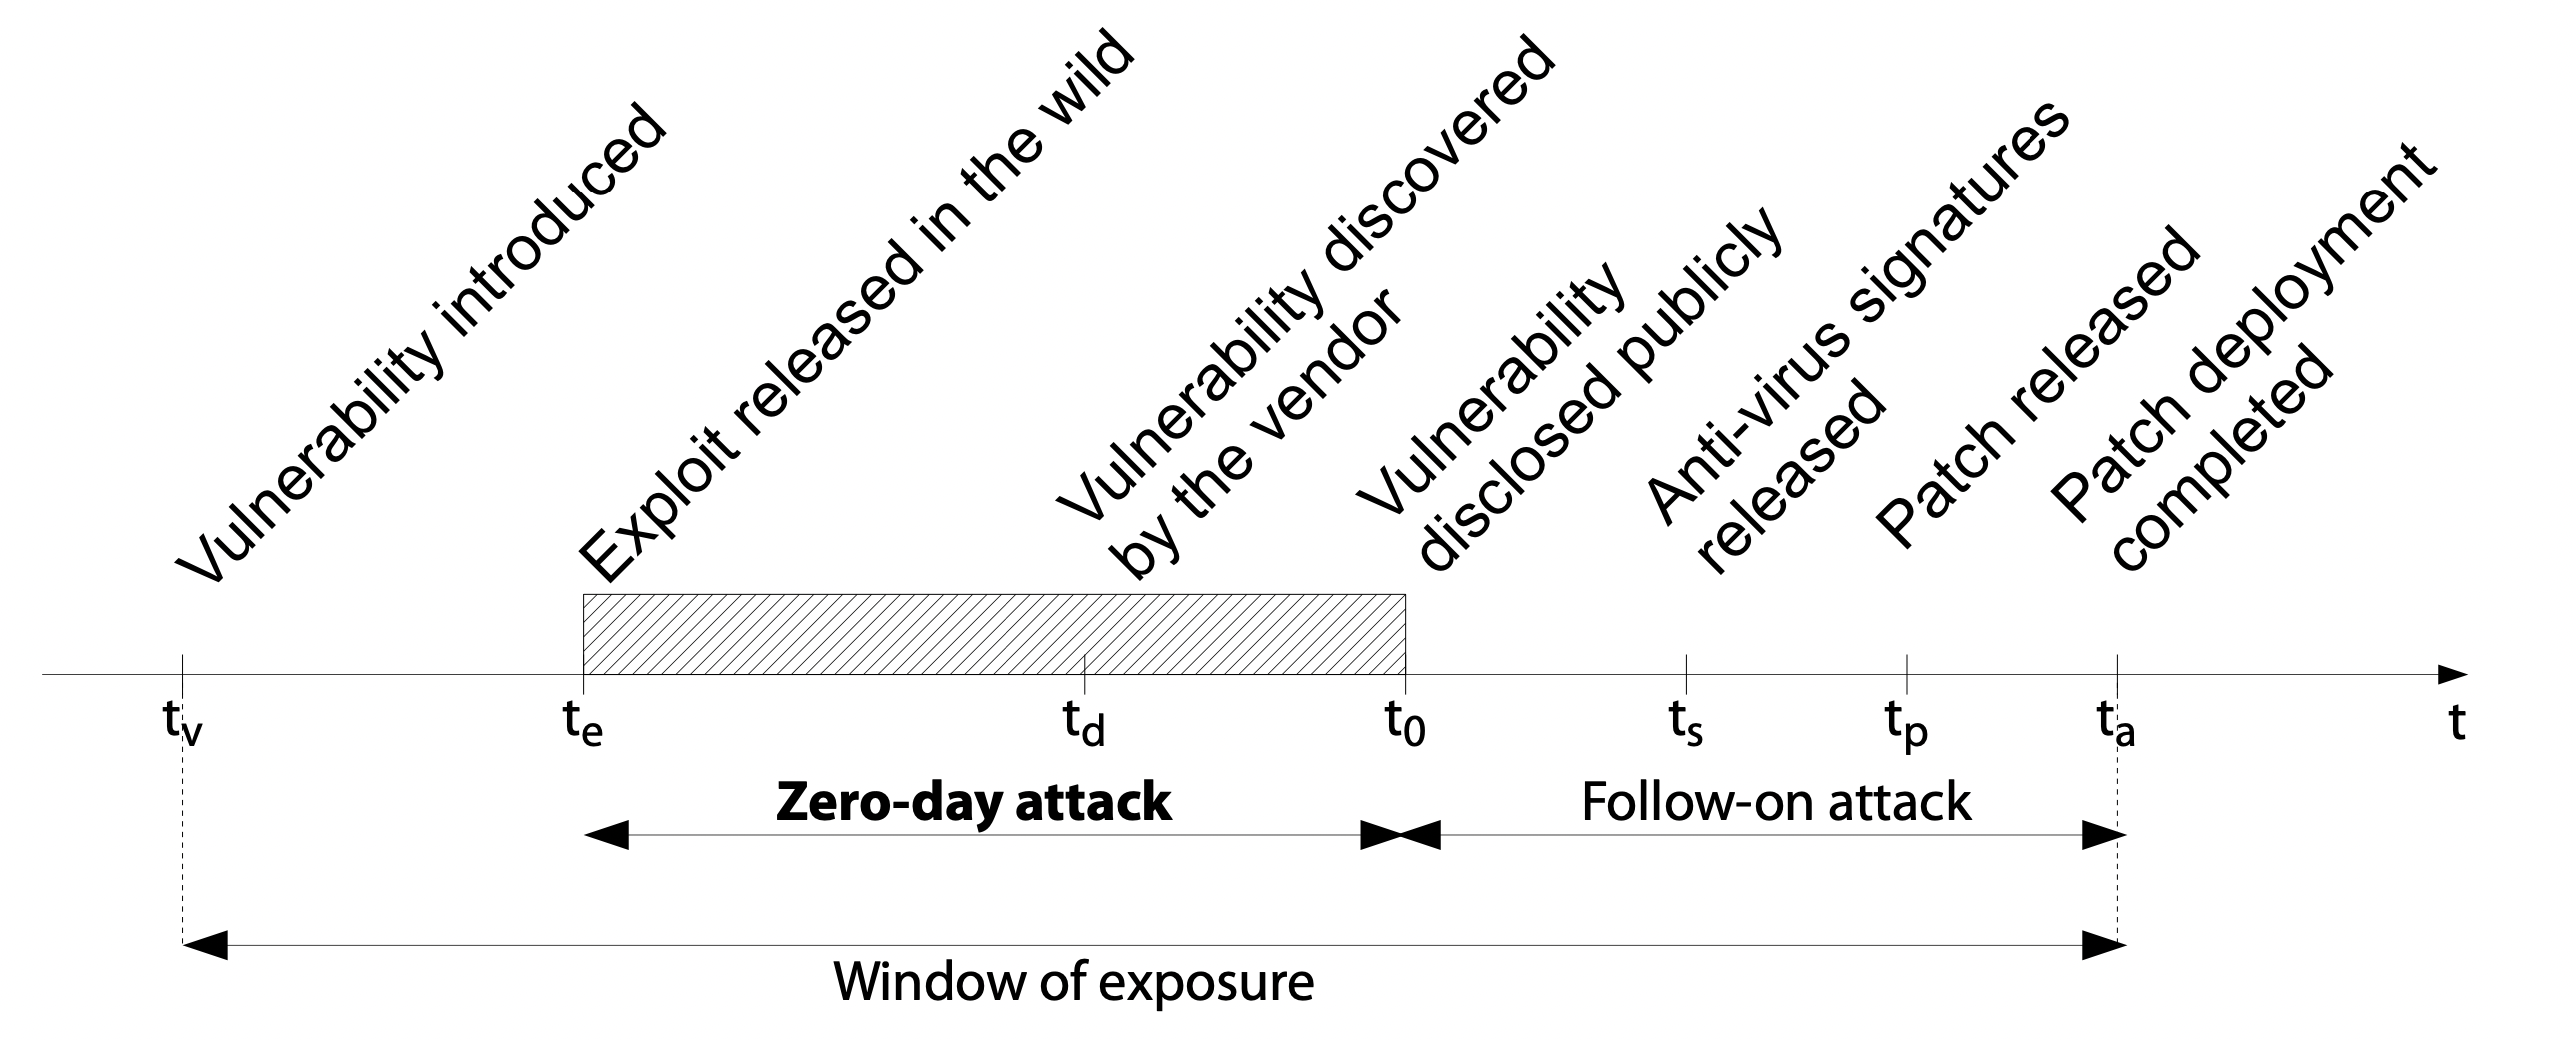
\includegraphics[width=0.90\textwidth]{imgs/vulnerability_windows.png}
    \caption{Sequenza degli eventi di una vulnerabilità}
    \label{fig:Sequenza degli eventi di una vulnerabilità}
  \end{flushright}
\end{figure}

In una tipica sequenza degli eventi di una vulnerabilità, le patch di 
sicurezza si installano a partire dal punto temporale tp 
(mostrato nella figura ~\ref{fig:Sequenza degli eventi di una vulnerabilità}), 
momento in cui il produttore rilascia al pubblico la risoluzione alla 
falla di sicurezza e inizia la campagna di aggiornamento, per risolvere la criticità. 
Durante questo periodo di patching (aggiornamento), che può durare anche 
mesi, il sistema, nella maggior parte dei casi, è ancora vulnerabile e 
solo una rapida installazione, della patch di sicurezza, può mettere il 
sistema informatico al riparo da un attacco che sfrutta quella falla.

Ed è proprio per installare rapidamente le patch di sicurezza che nasce 
l’Hotfix Response Center, nome ufficiale di questo progetto di tesi.
Lo scopo di questo strumento è quindi quello di gestire, in automatico, 
il patching straordinario di più server Linux o Windows Server che sono 
impattati dalla falla di sicurezza, per il quale è stata rilasciata 
la patch.
L’installazione delle patch di sicurezza avviene tramite la creazione 
di campagne di aggiornamento. Durante la creazione della 
campagna andranno specificati tutti i server impattati e dovranno essere 
caricate, all’interno del tool Hotfix, per ogni sistema operativo, le 
patch per risolvere le vulnerabilità, che il produttore avrà provveduto 
a rilasciare pubblicamente.

Questo strumento è indipendente da qualsiasi altro strumento ed è composto
da un’interfaccia grafica (frontend), da dei servizi REST (backend), da
un database dedicato, da uno storage per il caricamento delle patch e da
due script necessari all’installazione della patch di sicurezza, uno 
specifico per Windows, scritto in Powershell, e uno per Linux, scritto 
in bash.


\section{Funzionalità principali}
\subsection{Creazione di una campagna}
Una campagna di aggiornamento è un insieme di server, con diverso sistema 
operativo, che devono essere aggiornati, entro un periodo che va tra due e 
quattro settimane. 

\noindent Per creare una campagna occorre decidere:
\begin{itemize}
\item data e ora di inizio campagna;
\item data e ora di fine campagna;
\item elenco dei server impattati;
\item patch di sicurezza (rilasciate dal produttore del software) per 
ogni sistema operativo;
\end{itemize}
L’interfaccia grafica (frontend) per la creazione delle campagne sarà 
divisa in 3 step:
\begin{itemize}
\item Inserimento delle proprietà della campagna, tra cui: nome, data di 
inizio e fine, email del responsabile e tipologia della campagna 
(dettagliate più avanti).
\item Selezione dei server impattati: tramite le API (Application Program 
Interface) del gestionale in cui sono salvate tutte le informazioni dei 
server, si selezionano tutti i server impattati. L’interfaccia dovrà 
permettere di filtrare l’elenco completo dei server in base a: nome del
server, sistema operativo, indirizzo IP e tag associati ai server. 
Per tutti i server selezionati saranno poi recuperate tutte le informazioni
per consentire l’aggiornamento (dettagliate più avanti).
\item Caricamento delle patch: dopo aver selezionato tutti i server impattati,
per ogni sistema operativo selezionato, si dovrà caricare la patch di sicurezza 
da installare sui server.
\end{itemize}

\noindent Per ogni server da aggiornare bisogna recuperare, tramite le API del gestionale 
esterno, le seguenti proprietà:
\begin{itemize}
\item nome;
\item sistema operativo in uso;
\item indirizzo ip;
\item utenza di amministrazione per la connessione remota, utilizzata per 
installare le patch;
\item fascia di manutenzione: se presente indica le fasce orarie in cui il
server può essere aggiornato e riavviato. Ad esempio: MAR-MER-GIO(13:00-18:00)
indica che un server può essere aggiornato martedì, mercoledì e 
giovedì dalle 13 alle 18;
\item gruppo di patch: se presente impone che due o più server dello
stesso gruppo di patch non siano mai sotto manutenzione contemporaneamente. 
Questo per evitare problemi su applicazioni distribuite in cui tutti i server 
vengono aggiornati contemporaneamente. Chiamato con il campo restart group.
\item dipendenze: alcuni server devono essere aggiornati prima di altri. 
Ad esempio: i server di quality vanno aggiornati prima dei server di produzione.
Se un server ha una dipendenza bisogna fare in modo che durante l’aggiornamento
venga rispettata, garantendo almeno 24 ore tra una aggiornamento e l'altro.
\end{itemize}
Le credenziali per la connessione al server fornite devono essere funzionanti e con 
permessi di amministratore sulla macchina. Queste credenziali verranno usate
per la connessione remota al server.
Per consentire l’aggiornamento i server Windows devono avere WinRM abilitato.
Mentre i server Linux devono avere SSH attivo. WinRM è un protocollo di 
gestione usato da Windows per comunicare in remoto con un server. 
Si tratta di un protocollo che comunica su HTTPS, ed è incluso in tutti 
i recenti sistemi operativi Windows. Da Windows Server 2012, WinRM è 
abilitato di default. 
SSH, o Secure Shell, è un protocollo di amministrazione remota che consente 
agli utilizzatori di creare una connessione sicura con i server Linux.
WinRM e SSH verranno utilizzati attraverso Ansible per l’esecuzione di task
remoti. Il funzionamento di Ansible verrà approfondito a 
pagina ~\pageref{subsec:Ansible}.

\noindent Le campagne possono avere due tipologie:
\begin{itemize}
\item standard: in cui vengono rispettate le fasce di manutenzione impostare 
per ogni server;
\item zero day: in cui tutti i server vengono schedulati per essere 
aggiornati il prima possibile.
\end{itemize}


\subsection{Schedulazione intelligente dei server}
Durante la creazione della campagna, quando si selezionano i server impattati 
dalla vulnerabilità di sicurezza, è possibile selezionare anche tutti i server
inseriti nel gestionale. 
È quindi necessario creare un algoritmo di schedulazione efficiente, capace di 
distribuire tutti i server da aggiornare, durante il periodo della campagna.
Tutte le campagne di aggiornamento durano tra due e quattro settimane. 
Ogni giorno viene diviso in più slot di 30 minuti. L’algoritmo di schedulazione 
dovrà essere in grado di trovare una schedulazione ottimale in base ai 
seguenti parametri:
\begin{itemize}
\item fascia di manutenzione corretta;
\item dipendenze tra server;
\item schedulare in modo da non avere due server con lo stesso 
“gruppo di patch” nello stesso slot;
\item schedulare in modo da avere massimo di server per slot, preferendo 
sempre slot vuoti. In una situazione ideale si schedula solo 1 server per slot.
\end{itemize}
L’algoritmo di schedulazione dovrà essere eseguito appena l’operatore, tramite 
l’interfaccia grafica, avrà inserito tutti i server da aggiornare nella 
campagna. L’algoritmo ha quindi pochi secondi per reperire le informazioni 
necessarie dei server e trovare la schedulazione migliore per la campagna.
Al termine dell’elaborazione verrà mostrato all’operatore un calendario con
tutte le schedulazioni di tutti i server nella campagna.
Attraverso il calendario della campagna dovrà essere possibile cambiare la 
data e/o l’ora di schedulazione, nel caso l’operatore ritenga opportuno
cambiare alcune schedulazioni.


\subsection{Caricamento file di aggiornamento}
Dopo l’inserimento di tutti i server vulnerabili, all'interno della campagna 
di aggiornamento, ci sarà un schermata di caricamento dei file di aggiornamento.
In questa schermata, per ogni differente sistema operativo dei server
selezionati, verrà dinamicamente mostrato l’elenco dei sistemi operativi
e un’interfaccia di caricamento per l’eseguibile/script di aggiornamento, 
da lanciare sulla macchina.
I file che saranno caricati dall’operatore saranno salvati in uno storage 
S3 dedicato.
Terminato il caricamento delle patch, per ogni sistema operativo, la campagna 
di aggiornamento può essere attivata dall’operatore.


\subsection{Avvio aggiornamento automatico}
La gestione degli aggiornamenti dei server dovrà essere automatica. 
Gli automatismi saranno gestiti con due cron jobs. I cron jobs sono 
dei programmi che vengono eseguiti ad orari prestabiliti. Cron è un programma di
utilità dei sistemi di tipo Unix che consente agli utenti di gestire 
le pianificazione di attività ripetute in un momento specifico.
La gestione automatica degli aggiornamenti sarà quindi gestita con 
dei task programmati che faranno partire l’aggiornamento sul server remoto.\\

\noindent Saranno presenti due cron job:
\begin{itemize}
\item job di avvio, schedulato ogni 30 minuti. Questo job seleziona tutte 
le campagne attive e farà partire gli aggiornamenti per i server schedulati 
in quello slot temporale. Ad esempio il job che parte alle 13:30 farà 
partire l’aggiornamento per i server schedulati dalle 13:30 alle 13:59; 
\item job di monitoraggio, schedulato ogni 10 minuti. Questo job monitorerà gli 
aggiornamenti in corso. Deve controllare che gli aggiornamenti automatici
procedano senza problemi rilevando se si verificano dei timeout 
(l’aggiornamento sta durando troppo oppure qualcosa si è interrotto 
senza preavviso). Questo job deve inoltre monitorare il corretto riavvio 
dei server dopo l’aggiornamento, per considerare l’aggiornamento 
come completato.
\end{itemize}


\subsection{Gestore dell’aggiornamento}
Un’ultima parte molto importante di questo sistema è lo script che gestirà 
l’aggiornamento sulla macchina remota. Ci saranno due diversi script: 
uno per i server Linux e uno per Windows server.
Lo script per Linux sarà realizzato in Bash mentre lo script per Windows 
server sarà realizzato in Powershell. Entrambi sono linguaggi di 
programmazione adatti per creare script iterativi da eseguire nella 
console dei rispettivi sistemi.
Il compito di questo script sarà quello di gestire l'aggiornamento del 
server remoto in modo automatico, comunicando con il server centrale lo 
stato dell’aggiornamento.
Lo scopo è quindi quello di scaricare la patch di aggiornamento dallo 
storage centrale e far partire l’aggiornamento sul server.
Per avere un maggiore controllo sullo stato di avanzamento lo script 
comunicherà gli stati intermedi durante l’operazione.\\

\noindent Gli stati che si susseguiranno durante l’operazione saranno:
\begin{itemize}
\item ping: test connessione all’avvio dello script; 
\item download patch: scaricamento dell’aggiornamento sul server;
\item esecuzione: installazione dell’aggiornamento;
\item reboot: riavvio del server, se necessario.
\end{itemize}
Al termine del riavvio il job di monitoraggio assegnerà lo stato 
completato. Se trascorre troppo tempo in uno step intermedio 
l’installazione andrà in timeout e l’aggiornamento sarà fallito.
La figura di pagina ~\pageref{fig:Diagramma a stati dell'aggiornamento di un server}
mostra il diagramma degli stati dell'aggiornamento.

\section{Diagramma delle attività}
La figura ~\ref{fig:Diagramma delle attività per la creazione di una campagna} 
rappresenta il diagramma delle attività per la creazione di una campagna di Hotfix.\\

\noindent Le entità coinvolte nella creazione sono:
\begin{itemize}
\item NIST (National Institute of Standards and Technology);
\item Il vendor del sistema operativo cioè colui che ha creato e gestisce il 
sistema operativo (Esempio Microsoft è il vendor di Windows);
\item Il tool Hotfix Response Center;
\item Il cliente.
\end{itemize}

Il flusso che porta alla creazione di una campagna di installazione 
parte dal NIST, l’ente americano che si occupa di gestire il National 
Vulnerability Database (NVD) fornendo punteggi CVSS per tutte le 
vulnerabilità note. Per quasi tutte le vulnerabilità, i vendor si preoccupano 
di fornire un patch, per sanare la vulnerabilità.
Il tool Hotfix Response Center è stato pensato per intervenire in situazioni 
d'emergenza, per patchare nel più breve tempo possibile le vulnerabilità critiche. 
Nel caso il CVSS (Common Vulnerability Scoring System) superi lo score di 9 su 
10 si controlla se tra i server dei clienti è presente la vulnerabilità appena scoperta.

Se i server dei clienti sono impattati si informa il cliente e, nel caso autorizzi 
l’aggiornamento straordinario, si procede con la creazione della campagna di 
aggiornamento per i server impattati dalla vulnerabilità.

Durante la creazione della campagna vengono caricate le patch di aggiornamento 
all’interno del tool e l’algoritmo di schedulazione cerca di trovare una 
schedulazione ottimale per patchare i server, nel più breve tempo possibile. 
Al termine di queste operazioni la campagna può essere avviata.

Sarà poi compito del cronjob di avvio, che parte ogni 30 minuti, controllare 
tutte le campagne attive e far partire l'aggiornamento automatico per i server 
schedulati nelle varie fasce d'orario.

\begin{figure}[H]
  \begin{flushright}
    \centering
    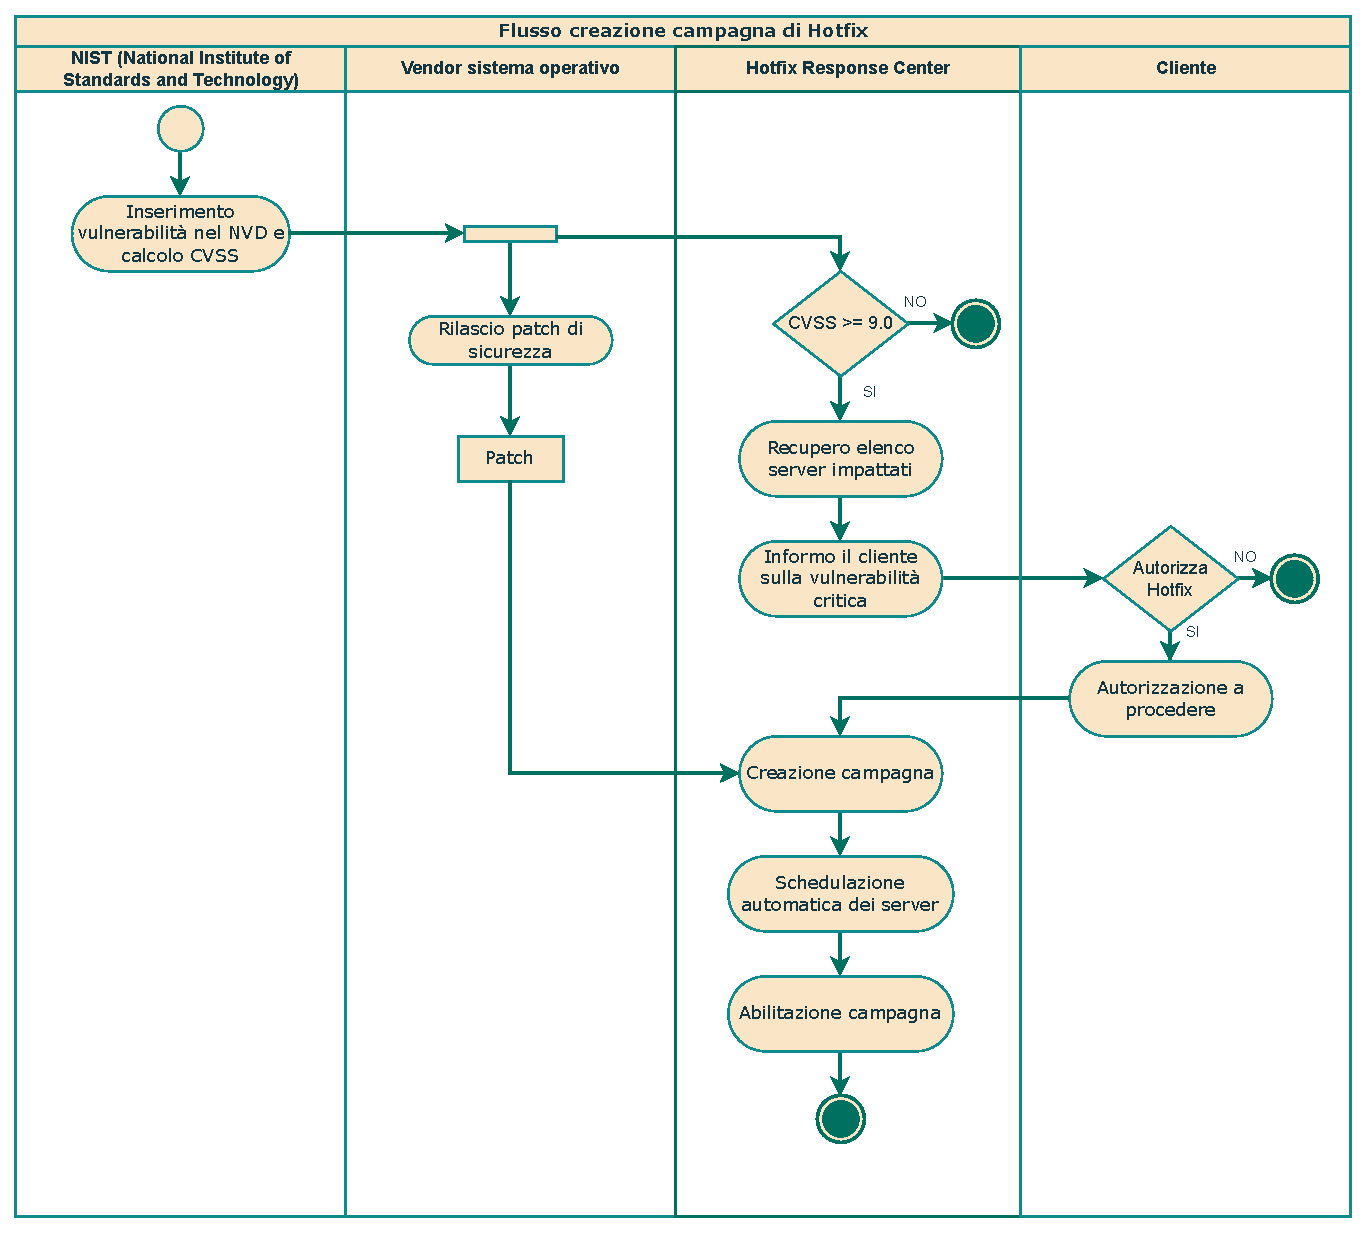
\includegraphics[width=0.98\textwidth]{imgs/hotfix_activity_diagram.pdf}
    \caption{Diagramma delle attività per la creazione di una campagna}
    \label{fig:Diagramma delle attività per la creazione di una campagna}
  \end{flushright}
\end{figure}
  \mcchap{Progettazione}{cap:cap3}
\section{Entità ed associazioni}
Nella fase di progettazione concettuale del tool, uno dei principali
obiettivi è stata la definizione di un modello di dati che potesse 
supportare le funzionalità principali dell'applicazione.
A tal fine, si è deciso di realizzare un database relazionale che 
contenesse diverse tabelle. La creazione delle tabelle è gestita 
tramite Django, un framework Python molto conosciuto nello sviluppo di 
applicativi backend, verrà dettagliato in seguito.\\

\noindent Il database relazionale comprende quindi diverse tabelle, tra cui:
\begin{itemize}
\item campaign: la tabella principale del database, che rappresenta una 
campagna di aggiornamento. Ogni record in questa tabella contiene 
informazioni sulle specifiche della campagna;
\item item: tabella che contiene l'insieme dei server che devono essere 
aggiornati, correlati alla campagna tramite una relazione uno-a-molti. 
Ogni record in questa tabella rappresenta un singolo server da aggiornare;
\item updatefile: tabella che contiene le informazioni sui file di aggiornamento 
effettivi che verranno installati sui server selezionati. 
Anche questa tabella è correlata alla tabella “campaign” tramite una 
relazione uno-a-molti e contiene un record per ogni diverso sistema 
operativo dei server selezionati in una campagna di aggiornamento;
\item updatejob: tabella che contiene le informazioni sulle sessioni 
di aggiornamento avviate su un server. Ogni record in questa tabella 
rappresenta un'operazione di aggiornamento. È possibile avere più operazioni 
di aggiornamento per un singolo server, per consentire di ripetere 
l’aggiornamento in caso di fallimento;
\item updatejobstatushistory: tabella che tiene traccia dello stato d'avanzamento 
dell’operazione di aggiornamento. Questa tabella è utilizzata 
per tenere traccia degli stati di ogni singola operazione di aggiornamento 
presente nella tabella.
\end{itemize}

\begin{figure}[H]
  \begin{flushright}
    \centering
    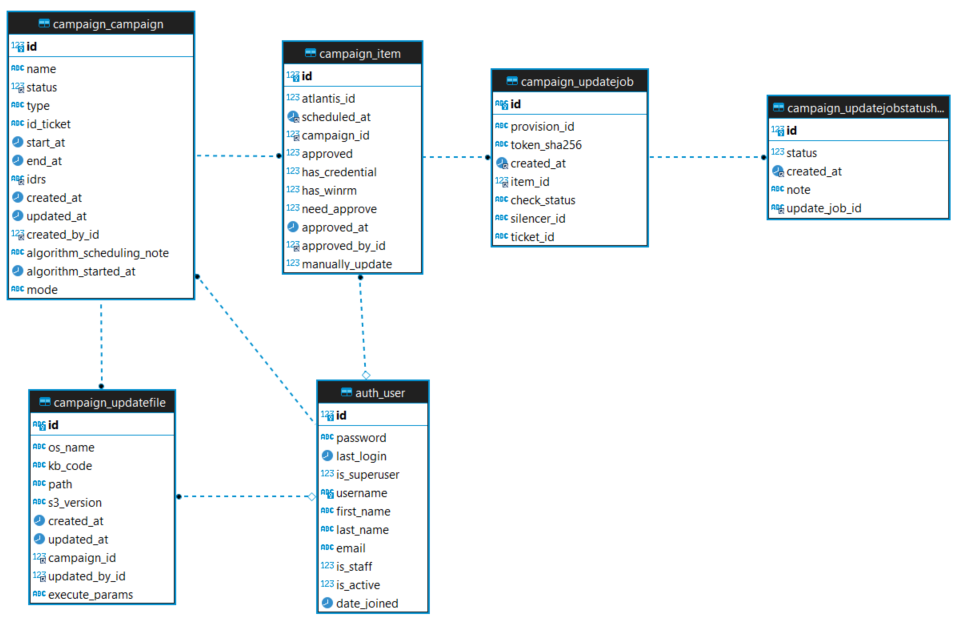
\includegraphics[width=0.95\textwidth]{imgs/ER_schema.png}
    \caption{Schema entità-relazione del database relazionale}
    \label{fig:Schema entità-relazione del database relazionale}
  \end{flushright}
\end{figure}

Come mostra lo schema ER della figura
~\ref{fig:Schema entità-relazione del database relazionale}, le tabelle del database sono state 
progettate in modo da riflettere le relazioni tra le entità coinvolte 
nel sistema.

La tabella “item” è correlata alla tabella “campaign” attraverso una 
relazione uno-a-molti, in quanto ad ogni campagna di aggiornamento 
corrisponde un insieme di server che devono essere aggiornati.

La tabella “updatefile” è sempre correlata alla tabella “campaign” 
attraverso una relazione uno-a-molti, in quanto ad ogni campagna di 
aggiornamento corrisponde un insieme di file che 
devono essere installati sui server selezionati.

La tabella “updatejob” è correlata alla tabella “item” in quanto ogni 
operazione di aggiornamento è associata ad un singolo server.

La tabella “updatefile” è associata alla tabella “campaign”, sempre 
attraverso relazioni uno-a-molti, perché in base al sistema operativo 
ogni server della campagna avrà il suo file di aggiornamento. 

La tabella “updatejobstatushistory” è correlata alla tabella 
“updatejob” tramite una relazione uno-a-molti, in quanto ad ogni 
operazione di aggiornamento corrisponde un insieme di stati di 
avanzamento dell'operazione.

Inoltre, nello schema, è presente la tabella auth\_user. 
Questa tabella è utilizzata da Django per gestire le utenze che 
utilizzano il backend. Infatti, ogni campagna creata è associata ad 
un creatore e ogni file di aggiornamento caricato è associato ad un 
utente che l’ha caricato.

\subsection{Definizioni delle tabelle}

\noindent \textbf{Campaign:}
\begin{itemize}
\item id: l'ID univoco della campagna;
\item name: il nome associato alla campagna;
\item status: lo stato della campagna, può essere draft (bozza), scheduled (pianificata), started (avviata) o closed (chiusa);
\item type: il tipo della campagna, può essere pkg (pacchetto) o cve;
\item mode: la modalità della campagna, può essere standard o zero day;
\item id\_ticket: l'ID del ticket associato alla campagna;
\item start\_at: la data e l'ora di inizio della campagna;
\item end\_at: la data e l'ora di fine della campagna;
\item idrs: l’ID del cliente a cui è associata la campagna;
\item created\_by: l'utente che ha creato la campagna;
\item algorithm\_started\_at: la data e l'ora di inizio dell'algoritmo di elaborazione;
\item algorithm\_scheduling\_note: una nota di pianificazione dell'algoritmo di elaborazione;
\item created\_at: la data e l'ora di creazione della campagna;
\item updated\_at: la data e l'ora di ultima modifica della campagna.\\
\end{itemize}

\noindent \textbf{Item:}
\begin{itemize}
\item id: l'ID univoco dell’item;
\item campaign\_id: l’ID della campagna associata all'elemento;
\item atlantis\_id: l'ID del gestionale CMDB sul quale sono salvate le informazioni del server;
\item scheduled\_at: la data e l'ora di pianificazione dell'aggiornamento;
\item has\_winrm: indica se il server ha WinRM abilitato, attraverso un check eseguito alla creazione della campagna;
\item has\_credential: indica se il server ha una credenziale associata, attraverso un check eseguito alla creazione della campagna;
\item approved: indica se l'elemento è stato approvato automaticamente (se need\_approve è False);
\item need\_approve: indica se l'elemento richiede approvazione;
\item manually\_update: indica se l'elemento deve essere aggiornato manualmente;
\item approved\_at: la data e l'ora di approvazione dell'elemento;
\item approved\_by: l'utente che ha approvato l'elemento.
\end{itemize}

\noindent \textbf{UpdateFile:}
\begin{itemize}
\item id: l'ID del file.
\item campaign\_id: l'ID della campagna associata all'aggiornamento;
\item os\_name: il codice del sistema operativo associato all'aggiornamento;
\item kb\_code: il codice univoco dell'aggiornamento di sicurezza;
\item execute\_params: i parametri di esecuzione dell'eseguibile di aggiornamento;
\item path: l'url del percorso del bucket su cui è stato caricato il file di aggiornamento;
\item updated\_by: l'utente che ha caricato il file di aggiornamento;
\item s3\_version: la versione di S3 del file di aggiornamento;
\item created\_at: la data e l'ora di creazione del file;
\item updated\_at: la data e l'ora di ultima modifica del file.
\end{itemize}

\noindent \textbf{UpdateJob:}
\begin{itemize}
\item id: campo UUID che rappresenta la chiave univoca della sessione di aggiornamento;
\item item\_id: l'ID che si riferisce al modello Item e specifica l'elemento di cui viene effettuato l'aggiornamento;
\item provision\_id: contiene l'ID del gestore dei task schedulati remoti, utilizzato per far partire l'aggiornamento da remoto;
\item token\_sha256: contiene il valore SHA256 del token utilizzato per inviare aggiornamenti di stato da remoto;
\item ticket\_id: campo che può contenere l'ID del ticket che viene aperto in caso di problemi di aggiornamento automatico;
\item check\_status: campo che contiene lo stato di tutti i controlli di monitoraggio, prima di avviare l'aggiornamento;
\item silencer\_id: l'ID del downtime associato al server per evitare segnalazioni dovute al riavvio della macchina durante l'aggiornamento;
\item created\_at: la data e l'ora dell'avvio dell'aggiornamento.
\end{itemize}

\noindent \textbf{UpdateJobStatusHistory:}
\begin{itemize}
\item update\_job\_id:  l'ID della sessione di aggiornamento;
\item status: specifica lo stato dell'aggiornamento. I possibili valori sono: “Ready”, 
“Execute error from provision”, “Waiting for ping”, “Timeout ping”, 
“Waiting for download process”, “Timeout download”, “Running”, “Timeout running”, “Rebooting”, 
“Failed”, “Completed”;
\item created\_at: la data e l'ora del passaggio di stato;
\item note: campo che contiene eventuali note aggiuntive per lo stato dell'aggiornamento.
\end{itemize}


\section{Design architettura}
L’Hotfix Response Center è stato realizzato con un’architettura a container. 
I container sono ambienti isolati e leggeri che includono tutto il necessario 
per eseguire un'applicazione, compresi il codice, le dipendenze e le librerie.

\subsection{Kubernetes}
La gestione dei container è affidata a Kubernetes, un sistema open-source per 
l'orchestrazione dei container. È progettato per automatizzare la distribuzione, 
la scalabilità e la gestione delle applicazioni containerizzate.

Kubernetes fornisce un'infrastruttura per coordinare e gestire il deployment 
dei container in modo efficiente. Si può definire come le applicazioni dovrebbero 
essere eseguite, specificando requisiti di risorse, definendo relazioni tra i 
componenti e gestendo le dipendenze.

Su Kubernetes, i container sono organizzati e gestiti all'interno di unità 
chiamate “pod”. Un pod è il più piccolo oggetto di gestione in Kubernetes e 
rappresenta un singolo insieme di uno o più container, con uno spazio di 
archiviazione e una rete condivisa.\\

\noindent Le principali caratteristiche di  Kubernetes sono:
\begin{itemize}
\item Orchestrazione: coordina e distribuisce i container su un cluster di macchine (insieme di server). Gestisce automaticamente il posizionamento dei container, il bilanciamento del carico, la scalabilità e il ripristino in caso di errori;
\item Autoscaling: supporta l'autoscaling automatico in base al carico dell'applicazione. Può aumentare o diminuire il numero di repliche dei container in base alle metriche definite, assicurando che l'applicazione abbia sempre le risorse necessarie per funzionare correttamente;
\item Gestione delle risorse: consente di definire i requisiti di risorse per i container, come CPU e memoria, e li alloca in modo appropriato all'interno del cluster. Ciò garantisce che le risorse siano utilizzate in modo efficiente e che le applicazioni non interferiscano tra loro;
\item Rolling updates e rollback: facilita gli aggiornamenti delle applicazioni senza interruzioni. Si possono eseguire aggiornamenti dei container in modo graduale e controllato, monitorando lo stato e, se necessario, effettuando il rollback a una versione precedente.
\end{itemize}

Le risorse dell’Hotfix Response Center sono tutte state inserite in un namespace 
dedicato (una sorta di contenitore virtuale) in modo da poter coesistere con 
altri microservizi all'interno del cluster.\\

\noindent All’interno del namespace dedicato sono presenti le seguenti risorse:
\begin{itemize}
\item Deployment frontend: esegue un pod con il web server nginx che mette a disposizione i file statici del front-end, relativo al pannello di amministrazione;
\item Deployment backend: esegue tre pod che consentono l’esecuzione del backend in Django;
\item Cronjob di avvio: schedulato ogni 30 minuti. Questo job seleziona tutte le campagne attive e fa partire gli aggiornamenti per i server schedulati in quello slot temporale;
\item Cronjob di monitoraggio: schedulato ogni 10 minuti. Questo job monitora gli aggiornamenti in corso. Deve controllare che gli aggiornamenti automatici procedano senza problemi rilevando se si verificano dei timeout.
\end{itemize}

La figura ~\ref{fig:Design architettura} 
mostra uno schema rappresentativo dell’architettura.

\begin{figure}[H]
  \begin{flushright}
    \centering
    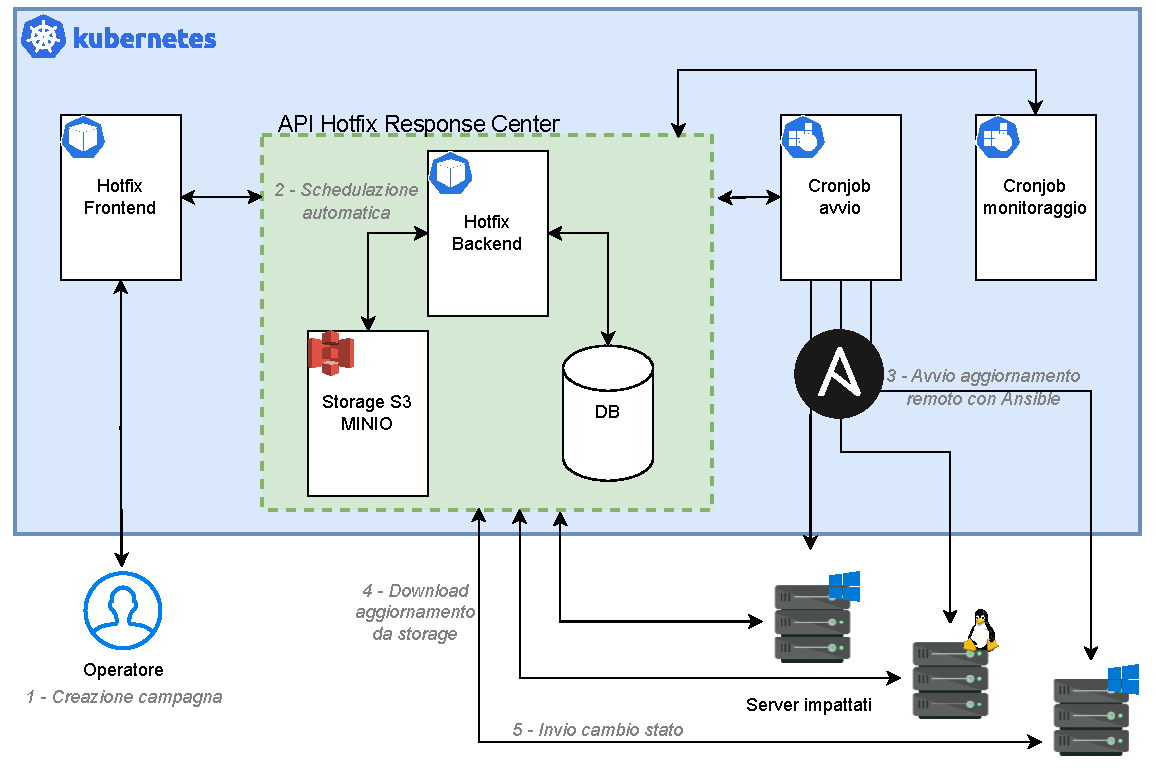
\includegraphics[width=0.95\textwidth]{imgs/architecture_design.pdf}
    \caption{Design architettura}
    \label{fig:Design architettura}
  \end{flushright}
\end{figure}

Il rettangolo azzurro rappresenta il namasepace dedicato all'interno del cluster.
Il backend contatta anche altri microservizi, presenti in altri namespace, dello stesso cluster.
Ad esempio contatta le API del gestionale per recuperare le informazioni dei server da aggiornare.

\label{subsec:Ansible}
\subsection{Ansible}
Un altro componente importante dell’architettura è Ansible, una piattaforma 
open-source per l'automazione IT. Ansible viene utilizzato per semplificare 
la gestione e l'automazione di sistemi IT complessi, utilizzando un 
linguaggio semplice basato su YAML chiamato “Playbook” per 
definire le azioni da eseguire sui nodi di destinazione.\\

Ansible viene utilizzato per connettersi da remoto ai server dei clienti per 
eseguire l’aggiornamento in modo automatico. Tramite Ansible viene lanciato un 
playbook sul nodo di controllo che, in base al sistema operativo del server da 
aggiornare, lancia un eseguibile per Windows o per Linux.
Questo eseguibile si occuperà dell'aggiornamento remoto del server. 
L’eseguibile, in modo autonomo, si preoccuperà di scaricare dallo storage 
S3 il file di aggiornamento e di installarlo sul server. 
Ad ogni passo d’esecuzione l’eseguibile comunica al backend dell’Hotfix Response Center, 
tramite le API, i passi dell’aggiornamento, seguendo lo schema di 
figura ~\ref{fig:Diagramma a stati dell'aggiornamento di un server}.

 \begin{figure}[H]
  \begin{flushright}
    \centering
    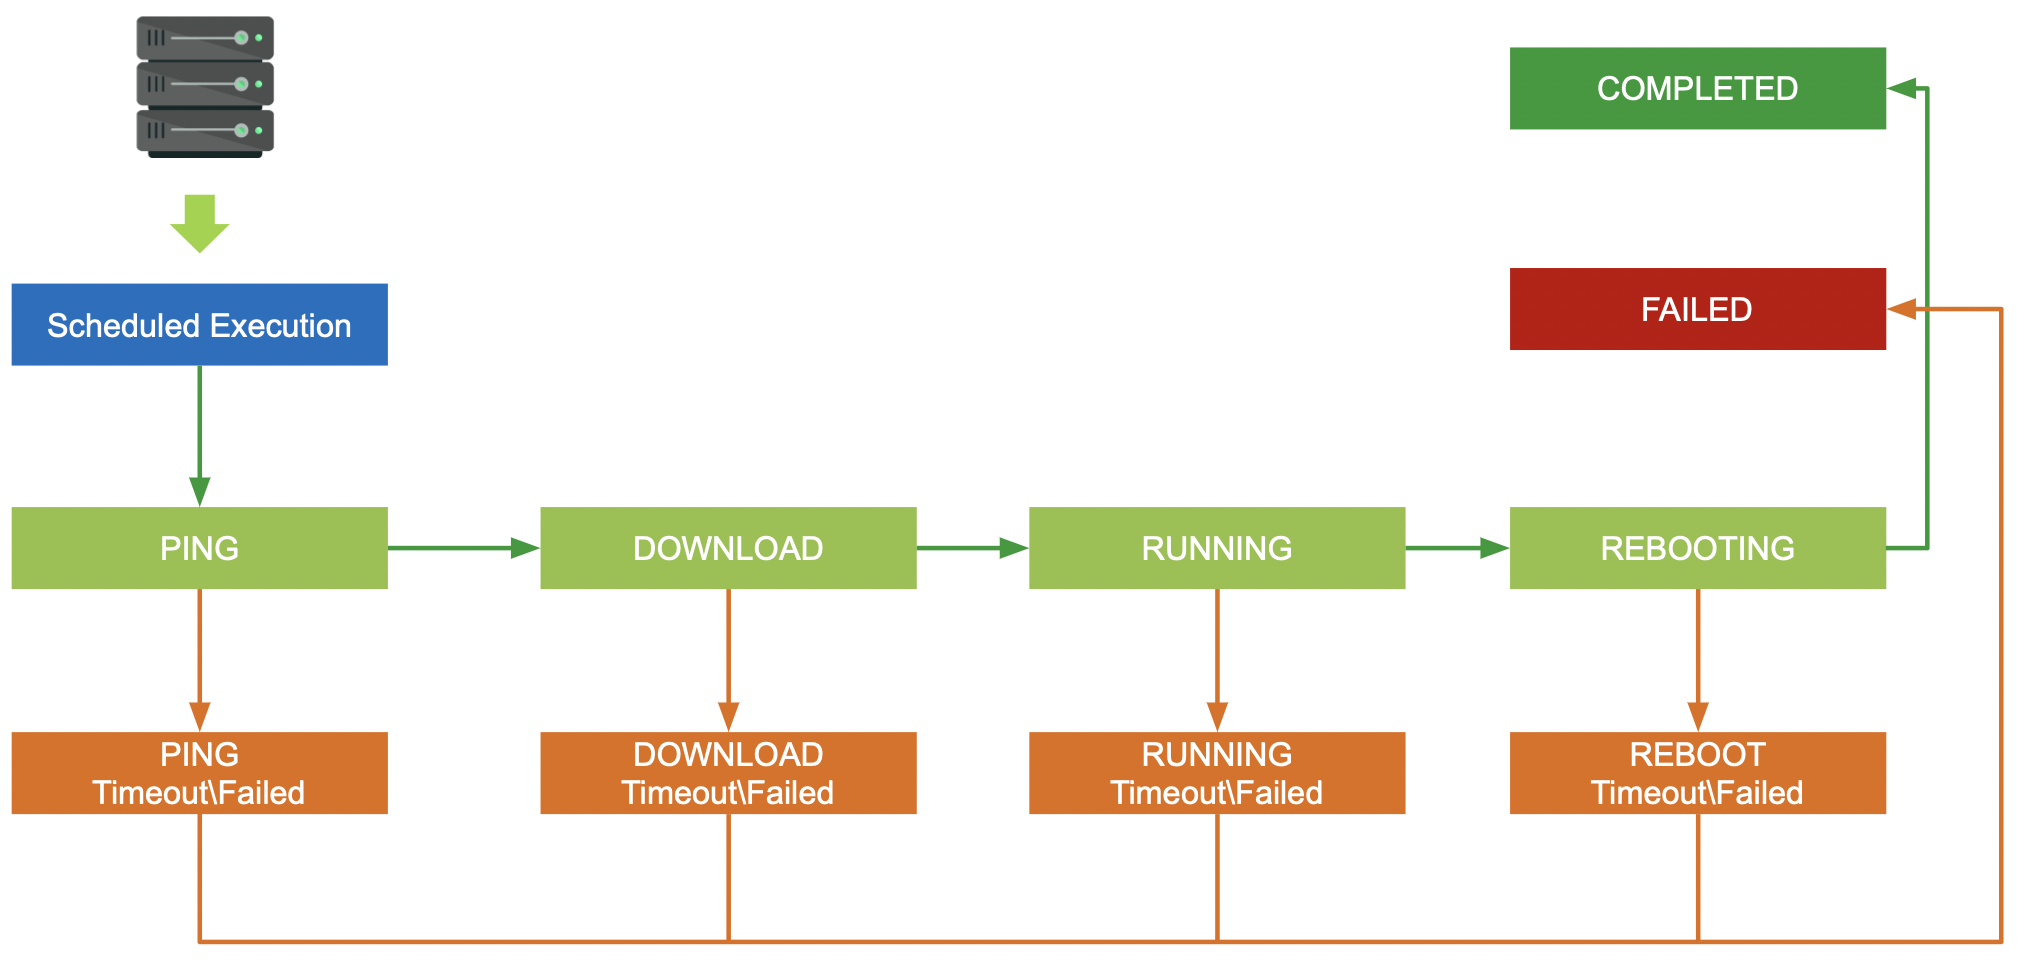
\includegraphics[width=0.90\textwidth]{imgs/update_statues.png}
    \caption{Diagramma a stati dell'aggiornamento di un server}
    \label{fig:Diagramma a stati dell'aggiornamento di un server}
  \end{flushright}
\end{figure}

Se l’aggiornamento avviene con successo il server andrà in stato “completed”.
Nel caso qualcosa non dovesse funzionare correttamente il cronjob di monitoraggio 
rileverà il timeout d’esecuzione e marcherà l’aggiornamento come “failed”.

  %%%%%%%%%% CAPITOLO DI TESI %%%%%%%%%%
%
% Capitolo "3" algoritmo di schedulazione
%
%%%%%%%%%%%%%%%%%%%%%%%%%%%%%%%%%%%%%%
\section{Algoritmo di schedulazione}
L’Hotfix Response Center è un tool che verrà utilizzato in momenti 
critici, per aggiornare da remoto centinaia di server vulnerabili, 
in modo automatico.

Ricopre quindi un ruolo molto importante l’algoritmo di schedulazione. 
L’algoritmo dovrà essere in grado di trovare una schedulazione 
ottimale per aggiornare i server tenendo conto, durante l'elaborazione, 
di numerosi fattori, dettagliati in seguito. L’affidabilità e la 
precisione dell’algoritmo sarà fondamentale per poter garantire che 
tutto avvenga in modo automatico e nelle corrette tempistiche.\\

La schedulazione avverrà generalmente su un periodo temporale 
di 2/3 settimane. Ogni giorno della settimana verrà suddiviso in 48 
slot da 30 minuti. Per ogni slot di tempo sarà possibile aggiornare 
massimo 5 server contemporaneamente. Questo rende possibile aggiornare 
fino a 240 server al giorno. La scelta di posizionare più server nello 
stesso slot dovrà avvenire solamente nel caso non ci siano altri slot 
liberi, preferendo sempre slot vuoti. In una situazione ideale si schedula 
solo 1 server per slot, questo per garantire uniformità nel calendario.\\

\textbf{Dati in input:} data e ora di inizio e fine campagna, elenco dei 
server da schedulare dove per ogni server sono presenti:
\begin{itemize}
\item atlantis\_id: id del gestionale dal quale provengono le informazioni del server;
\item fascia di manutenzione/aggiornamento;
\item gruppo di patch: duo o più server con lo stesso gruppo di patch non possono 
essere schedulati insieme;
\item dipendenze tra server. Questi server devono essere i primi ad essere 
schedulati a distanza di 24 ore.
\end{itemize}

\textbf{Dati in output:} schedulazione per ogni server in modo da poterli 
aggiornare il prima possibile.


\subsection{Concetto di euristica}
L’algoritmo realizzato per la schedulazione si basa su un principio euristico. 
Un'euristica è una tecnica o un metodo basato sull'esperienza o sulla 
conoscenza generale del problema, che cerca di trovare una soluzione 
ragionevole in tempi ragionevoli, anche in presenza di problemi di 
complessità elevata. In altre parole, un'euristica è un approccio basato 
sul buon senso, sulla logica e sulla creatività che, seppur non garantisca la 
soluzione ottimale del problema, può fornire risultati accettabili in tempi 
ragionevoli. Le euristiche sono spesso utilizzate per risolvere problemi di 
ottimizzazione in cui il tempo di calcolo richiesto per trovare una soluzione 
ottimale è troppo elevato.\\

Nel caso in questione l’algoritmo di schedulazione non esplora tutti i possibili 
casi per trovare la soluzione migliore ma si basa su dei calcoli preliminari 
per decidere quali server schedulare per primi.
Questa tecnica permette di ridurre drasticamente il tempo di esecuzione 
dell’algoritmo ottenendo un tempo di esecuzione lineare e fornendo una 
soluzione ottimale per creare un calendario di schedulazione per l’aggiornamento.\\

L’euristica si baserà sul calcolo dell’“availability score” che verrà utilizzato 
per decidere con che ordine schedulare i server all’interno del calendario.

È appropriato utilizzare un’euristica in quanto il calcolo della soluzione 
ottimale, che controllerebbe tutte le possibili schedulazioni, richiederebbe un 
tempo di esecuzione quadratico. Il calcolo e l’utilizzo del “availability score” 
per la schedulazione richiederebbe una complessità lineare in termini di tempo e 
spazio che fornirebbe una soluzione accettabile nel minor tempo possibile.


\subsection{Fascia di manutenzione}
Anche chiamata fascia di aggiornamento se presente indica le fasce orarie 
in cui il server può essere aggiornato e riavviato. 
Ad esempio: MAR-MER-GIO(13:00-18:00) indica che un server può essere 
aggiornato martedì, mercoledì e giovedì dalle 13 alle 18.
Se la fascia di manutenzione non è presente il server può sempre essere aggiornato.

La fascia di manutenzione è rappresentata da una stringa che deve essere 
interpretata correttamente prima di poter eseguire l’algoritmo di schedulazione. 

I giorni della settimana sono rappresentati dalle stringhe: 
LUN, MAR, MER, GIO, VEN, SAB, DOM. Seguiti dalla fascia oraria tra parentesi.
Una fascia di manutenzione può anche essere composta da più blocchi di fasce 
orarie, concatenati dal carattere +, come in questo esempio: 
LUN-MAR-MER(20:00-24:00)+LUN-MAR-MER(00:00-05:00)+SAB-DOM(00:00-24:00)\\

Per poter interpretare correttamente la stringa e capire durante la settimana in quali 
slot di 30 minuti può essere inserito il server è stata creata una classe 
Python capace di comprendere il significato della stringa.

Le funzionalità principali della classe sono:
\begin{itemize}
\item Interpretare la stringa della fascia di manutenzione;
\item Gestire una struttura dati per memorizzare in quali slot durante la 
settimana il server può essere in manutenzione;
\item Esporre un metodo che comunica se il server è in manutenzione in un 
determinato slot. Questo metodo verrà poi utilizzato dall’algoritmo di schedulazione.
\end{itemize}

La classe interpreta la stringa utilizzando delle regex (abbreviazione di 
"regular expressions", ovvero "espressioni regolari" in italiano) in grado di 
riconoscere pattern di testo ed eseguire successivamente gli opportuni calcoli.
La struttura dati per memorizzare la disponibilità degli slot si basa su un 
dizionario in cui la chiave del dizionario è la rappresentazione a stringa 
dell’inizio dello slot in secondi.

\textbf{Esempio:}\\
Chiave 0 = primo slot, lunedì mattina alle ore 00:00\\
Chiave 1800 = secondo slot, lunedì mattina alle ore 00:30\\
Chiave 86400 = slot del martedì alle ore 00:00\\

Questi valori sono ottenuti impostando la costante RESOLUTION\_IN\_MINUTE = 30. 
Quindi durante la settimana, nel dizionario, saranno presenti 336 slot da 30 minuti.

Dopo aver inizializzato la struttura dati, per salvare le disponibilità negli 
slot, inizia l’interpretazione della stringa della fascia di manutenzione.\\

Di seguito è riportato il metodo calc\_available\_slots presente all'interno della classe MaintenanceWindowParser:

\lstinputlisting[style=custompython, language=Python]{code/calc_available_slot.py}

Al termine dell’esecuzione il dizionario contenuto in self.data conterrà 336 chiavi. 
Ad ogni chiave è associato un valore booleano. Se il valore corrisponde a True il 
server è disponibile in quello slot per l’aggiornamento.


\subsection{Calcolo dello score}
Dopo aver trovato per ogni server quali sono gli slot disponibili durante la 
settimana si procede con il calcolo dell’“availability score” di ogni server. 
Questo valore numerico sarà utilizzato per decidere quali server andranno schedulati per primi.

L'Availability score corrisponde al numero di secondi in cui il server è disponibile 
per l’aggiornamento durante la settimana.
Più lo score sarà basso e meno slot ha un server a disposizione per essere aggiornato.\\

Attraverso l’approccio euristico è stato constatato che schedulando per primi i 
server con un availability score più basso non si compromette la schedulazione degli 
altri server. Non risulterà quindi necessario provare ogni possibile schedulazione 
per trovare la migliore ma ci si potrà accontentare della schedulazione deterministica 
che verrà creata assegnando prima i server con score più basso negli slot in cui 
possono essere aggiornati.
I server che saranno schedulati per ultimi saranno quelli con score più alto.
Questo significa che tali server potranno probabilmente essere schedulati 
negli slot lasciati liberi dai server con score più basso.\\


Di seguito è riportato il metodo get\_num\_of\_seconds\_of\_available\_slot della 
classe MaintenanceWindowParser:

\lstinputlisting[style=custompython, language=Python]{code/get_num_of_seconds_of_available_slot.py}


\subsection{Albero delle dipendenze}
Prima dell’esecuzione dell’algoritmo di schedulazione dovrà essere creato 
l’albero delle dipendenze, per i server con dipendenze, cioè che necessitano 
che un server venga aggiornato prima di eseguire l’aggiornamento del server 
stesso. Questi server saranno schedulati per primi, tenendo una distanza di 24 
ore tra uno slot e l’altro.

La struttura utilizzata è un albero. Alla radice è presente un nodo padre. 
I figli di primo livello sono tutti i server che non hanno dipendenze ma che 
fanno dipendere altri server.
I figli di secondo livello sono i server che dipendono dai server di primo livello
che dovranno essere aggiornati 24 ore dopo l'aggiornamento con successo dei filgi 
di primo livello, e così via\dots

L’albero viene gestito da una semplice classe Python, che viene popolata durante 
lo scorrimento preliminare di tutti i server.


\subsection{Esecuzione dell’algoritmo}
L’algoritmo di schedulazione risultante è abbastanza semplice. 
Si inizia con il calcolare il priority score di ogni server.
Questo valore è la somma tra l’availability score e il grado che 
ha il server all'interno dell’albero delle dipendenze, se i server non 
hanno dipendenze avranno grado 0.

Poi si ordinano i server per priority score crescente (riga 7).
Successivamente, nel ciclo for di riga 14, si scorrono tutti i server 
da schedulare presenti nella campagna.
Per ogni server si estrae la lista di tutti gli slot per cui provare 
la compatibilità. Questi slot da provare vengono restituiti dal metodo 
get\_list\_of\_slot\_to\_try (riga 19). Questo metodo restituisce gli slot 
in ordine temporale restituendo però prima gli slot che hanno meno server 
già assegnati.
Per ogni slot restituito si controlla, se è compatibile con la fascia di 
manutenzione del server (riga 21). Se la fascia di manutenzione permette 
l’utilizzo di quello slot il server viene schedulato altrimenti si prova 
per tutti gli slot rimasti.

Nel caso non ci sia nessuno slot disponibile, per effettuare 
l’aggiornamento del server, questo non avrà una schedulazione e non sarà 
inserito a calendario (riga 31). In questo caso l’operatore, prima 
dell’avvio della campagna, dovrà selezionare manualmente uno slot per 
schedulare il server.\\

Codice parziale dell'algoritmo di schedulazione:
\lstinputlisting[style=custompython, language=Python]{code/scheduling.py}


\subsection{Complessità e caso peggiore}
La complessità computazionale in tempo dell'algoritmo di schedulazione dipende 
principalmente dalla dimensione dell'input, cioè il numero di server da 
schedulare e il numero di slot di manutenzione disponibili (in base alla 
lunghezza in giorni della campagna).
L'algoritmo inizia ordinando i server in base al punteggio di priorità 
calcolato per ciascuno di essi, e poi prosegue scorrendo tutti i server in 
ordine di priorità crescente cercando di trovare uno slot di manutenzione 
valido per ciascuno. La complessità in tempo è dell'ordine di O(N*M), 
dove N è il numero di server e M è il numero di slot di manutenzione 
disponibili.\\

Per quanto riguarda la complessità in spazio, l'algoritmo utilizza un 
ammontare di memoria proporzionale alla dimensione dell'input, in quanto deve 
mantenere in memoria la lista dei server e il calendario degli slot di 
manutenzione. La quantità di memoria richiesta non dovrebbe essere un 
problema per input di dimensioni moderate, poiché la lista dei server e 
il calendario non dovrebbero essere eccessivamente grandi. Quindi la 
complessità in spazio dell'algoritmo è O(N).\\

L’algoritmo di schedulazione ha un comportamento computazionale in 
tempo lineare. Il caso peggiore non si verifica quando ci sono tanti 
server da schedulare ma quando ci sono molti server con una fascia di 
manutenzione molto ristretta, che quindi andrebbero tutti schedulati in 
pochi slot. Questo farebbe riempire gli slot di una particolare fascia di 
manutenzione o di un gruppo di slot. A quel punto i server si ritroveranno, 
al termine dell’esecuzione dell’algoritmo, senza uno slot assegnato. 
In questo caso l’utilizzatore del tool dovrà inserire manualmente uno slot, 
attraverso l’interfaccia, prima di avviare la campagna.\\

Per evitare di incorrere in troppi server senza schedulazione si è deciso di 
fissare il limite massimo di 2000 server per singola campagna di aggiornamento.


\subsection{Tempi di esecuzione}
L’algoritmo di schedulazione viene eseguito quando l’utente, attraverso 
l’interfaccia grafica dell’Hotfix Response Center, seleziona i server da 
aggiornare. A quel punto si hanno a disposizione pochi secondi per salvare 
l’elenco dei server a database, recuperare le informazioni per la schedulazione 
ed eseguire l’algoritmo.
Tutte queste operazioni sono eseguite da un servizio REST, sviluppato in Django, 
presente nel Backend.

Il tempo di risposta del servizio e quindi il tempo di attesa dell’utente è 
la somma di: tempo di salvataggio a database di un record di tipo Item per 
ogni server della campagna, tempo di recupero delle informazioni necessarie 
alla schedulazione (fascia di manutenzione e altri parametri) tramite le API 
dei microservizi del gestionale, tempo di esecuzione dell'algoritmo di 
schedulazione, tempo di salvataggio a database delle schedulazioni di ogni 
server e tempo di invio della risposta al client.

La Tabella Tab.~\ref{tab:algo-exec} mostra i tempi, in secondi, di esecuzione 
dell'algoritmo di schedulazione per diversi quantitativi di server. Come si 
può vedere, il tempo di schedulazione varia a seconda del numero di server 
coinvolti nella campagna. Il tempo di recupero delle informazioni necessarie 
alla schedulazione e il tempo di esecuzione dell'algoritmo sono i principali 
fattori che contribuiscono alla durata totale dell'operazione. In particolare, 
il recupero delle informazioni richiede più tempo per i numeri di server più 
elevati, mentre il tempo di esecuzione dell'algoritmo è relativamente costante. 
In generale, il servizio REST in Django presente nel Backend riesce a gestire 
l'operazione in pochi secondi, garantendo un'esperienza utente fluida.\\

\begin {table}[H]
\begin{center}
\begin{tabular}{|c|c|c|c|c|}
  
  \hline
  \rowcolor[gray]{.66}
  \textbf{Server} & \textbf{Schedulazione} & \textbf{Recupero info} & \textbf{Con dipendenze} & \textbf{Schedulati}\\
  
  \hline
  \rowcolor[gray]{.87}15 & \textbf{0,150} & 0,55 & 0 & 15 \\
  \rowcolor[gray]{.95}100 & \textbf{0,185} & 1,42 & 0 & 100 \\
  \rowcolor[gray]{.87}250 & \textbf{0,329} & 3,19 & 0 & 250 \\
  \rowcolor[gray]{.95}400 & \textbf{0,487} & 4,37 & 31 & 398 \\
  \rowcolor[gray]{.87}500 & \textbf{0,647} & 5,56 & 57 & 495 \\
  \hline
\end{tabular} 
\caption {Tempo di esecuzione algoritmo, tempi in secondi} \label{tab:algo-exec}
\end{center}
\end{table}


La colonna “con dipendenze” mostra, per la relativa campagna di test, quanti 
erano i server che dipendevano da altri server per l’aggiornamento. Nel caso 
della campagna con 500 server c’erano 57 server con dipendenze.

L’ultima colonna “schedulati” mostra il numero effettivo di server che 
l’algoritmo è riuscito a schedulare.\\

Nella campagna con 500 server 
l’algoritmo di schedulazione è riuscito a trovare in 0,647 secondi uno slot 
di schedulazione per 495 server. I 5 server rimanenti andranno schedulati a 
mano, attraverso l’interfaccia grafica del tool. Nel caso in questione i 5 server 
rimasti fuori hanno una fascia di manutenzione molto ristretta che è stata 
occupata da altri server con una fascia di manutenzione simile.

  \mcchap{Implementazione}{cap:cap4}
\section{Backend}
Il backend è la parte del sistema che si occupa dell'elaborazione dei dati e 
dell'interazione con il database. È responsabile della gestione delle 
richieste e delle risposte tra il frontend e il database.

Nel caso dell’Hotfix Response Center il backend è stato sviluppato 
utilizzando il framework Django, per Python. Django è stato utilizzato assieme 
alla libreria Django REST Framework per realizzare le API REST necessarie per 
la comunicazione tra frontend e backend.


\subsection{Api rest}
Le API REST (Representational State Transfer) sono un tipo di architettura 
software utilizzata per la progettazione e lo sviluppo di servizi web. 
Le API REST consentono alle applicazioni di comunicare tra loro e 
scambiare dati utilizzando i protocolli standard del web, come HTTP. 
Le API REST sono basate su un insieme di principi fondamentali. 
In primo luogo, utilizzano le risorse come concetto centrale, dove ogni 
risorsa rappresenta un'entità specifica (ad esempio, un oggetto, un 
utente, una transazione) e viene identificata da un URL univoco.

Le API REST utilizzano metodi HTTP come GET, POST, PUT, PATCH e DELETE 
per consentire alle applicazioni di accedere, creare, modificare o 
eliminare le risorse. Ad esempio, una richiesta HTTP GET a un'API REST 
può essere utilizzata per ottenere i dettagli di una risorsa, mentre una 
richiesta POST può essere utilizzata per creare una nuova risorsa.
Le API REST utilizzano anche la rappresentazione dei dati, di solito nel 
formato JSON o XML, per trasmettere le informazioni tra client e server. 
Questo permette una facile interoperabilità tra diverse piattaforme e 
linguaggi di programmazione.

Uno dei vantaggi delle API REST è la loro scalabilità e flessibilità. 
Le API REST sono state progettate per essere stateless, il che significa 
che ogni richiesta deve contenere tutte le informazioni necessarie per 
essere elaborata e non richiede lo stato persistente del server. Ciò 
consente una maggiore scalabilità del sistema e la possibilità di 
distribuire le risorse su più server. ~\cite{wiki:api_rest}\\


\subsection{Django}
\label{subsec:Django}
Django REST Framework, spesso abbreviato in DRF, è un framework 
open-source per lo sviluppo di API REST. Offre una serie di funzionalità 
che semplificano la creazione di API scalabili e ben documentate.
DRF si basa sui concetti fondamentali di Django, come il modello 
MVC (Model-View-Controller) e l'ORM (Object-Relational Mapping). 
Sfrutta la potenza di Django per fornire una struttura solida e coerente 
per la creazione di API REST. Con DRF, è possibile definire i modelli di 
dati utilizzando le classi Django (che verranno poi convertiti in tabelle).

Una delle caratteristiche chiave di DRF è la sua gestione avanzata della 
serializzazione dei dati. Questo consente di convertire facilmente gli 
oggetti Python in formati serializzati come JSON o XML e viceversa. 
DRF offre anche un sistema completo per la gestione dell'autenticazione 
e dell'autorizzazione delle API. È possibile configurare facilmente 
l'autenticazione basata su token, l'autenticazione OAuth2, l'autenticazione 
basata su sessione e altre modalità di autenticazione. Inoltre, supporta la 
definizione di permessi personalizzati per controllare l'accesso agli 
endpoint delle API in base a regole specifiche.

Un'altra caratteristica utile di DRF è la gestione delle route API. 
DRF offre un sistema di routing che consente di definire 
facilmente gli endpoint delle API e associarli alle corrispondenti view. 
Questo semplifica l'organizzazione delle API in base a risorse specifiche 
e facilita la creazione di endpoint RESTful standardizzati.
Infine, DRF include un modulo di documentazione automatica che genera 
automaticamente la documentazione delle API basandosi sulle definizioni 
delle API e dei serializer. Questo rende più semplice per gli sviluppatori 
e gli utenti delle API comprendere e utilizzare correttamente le risorse 
fornite dall'applicazione. ~\cite{wiki:django}\\


\subsection{Esempio}
I seguenti pezzi di codice illustrano in Django la realizzazione di 
un'API REST per la gestione delle campagne all'interno del backend.
In particolare, l'esempio illustra come definire un modello di dati per una 
campagna, creare URL per gestire le richieste relative alle campagne, definire 
una vista che si occupa di recuperare e creare campagne utilizzando il modello 
e serializzare i dati della campagna utilizzando un serializer.

\lstinputlisting[style=custompython, language=Python]{code/django.py}

Nel file models.py viene definita la classe Campaign che estende la classe 
models.Model. Questa classe rappresenta il modello di dati per una campagna e 
contiene tutti i campi definiti nel paragrafo ~\ref{subsec:Definizioni delle tabelle} 
relativo alla definizione delle tabelle. 
Ogni campo definisce il tipo di dati che può contenere e le 
eventuali opzioni di configurazione. 

Nel file views.py viene definita la classe CampaignListCreateAPIView che 
gestisce le richieste relative alle campagne. La variabile queryset definisce 
l'insieme di dati su cui operare, in questo caso tutte le campagne ordinate per 
l'ID. Vengono anche specificati i  filtri e l’ordinamento da utilizzare. 
La variabile serializer\_class definisce la classe del serializer da utilizzare 
per la serializzazione dei dati in JSON. 
Questa vista estende la classe generics.ListCreateAPIView 
fornita da Django REST Framework e fornisce funzionalità per visualizzare 
l'elenco delle campagne e creare una nuova campagna.

Nel file serializers.py viene definita la classe CampaignSerializer che gestisce 
la serializzazione dei dati della campagna. La classe Meta all'interno del 
serializer specifica il modello di riferimento (Campaign), i campi da includere 
nella serializzazione ('\_\_all\_\_' indica tutti i campi del modello) e i campi di 
sola lettura che non possono essere modificati.

Nel file urls.py viene definito il percorso delle API per gestire le richieste 
relative alle campagne. In particolare, quando viene inviata una richiesta all'endpoint 
/campaigns/, viene utilizzata la classe CampaignListCreateAPIView come vista 
per gestire la richiesta.\\

Facendo richieste di HTTP GET sull’endpoint /campaigns/ verrà fornito l’elenco 
delle campagne inserite nel database. Sarà possibile utilizzare i filtri 
come queryparams della richiesta per 
ricercare tra tutte le campagne solo quelle desiderate. Le informazioni saranno 
restituite in formato JSON con i campi definiti nel serializer.

Facendo invece una richiesta di HTTP POST sullo stesso endpoint sarà possibile 
creare una nuova campagna. Le informazioni della nuova campagna andranno 
inserite nel body della richiesta.
Per entrambe le richieste dovrà essere fornito il token di autenticazione per 
verificare l’identità e le autorizzazioni dell’utente che sta utilizzando i 
servizi.


\section{Frontend}
Il frontend è la parte dell’applicazione che interagisce direttamente con 
l’operatore. È responsabile della presentazione dei dati consentendo agli 
utenti di visualizzare e interagire con il contenuto dell'applicazione web.

Nel contesto dello sviluppo web, il frontend si riferisce alla combinazione 
di tecnologie, linguaggi di programmazione e strumenti utilizzati per creare 
l'interfaccia utente di un'applicazione web. Ciò include l'utilizzo di HTML 
(Hypertext Markup Language) per definire la struttura e il contenuto della 
pagina, CSS (Cascading Style Sheets) per definire il layout e l'aspetto 
visivo della pagina, e JavaScript per aggiungere interattività e funzionalità 
dinamiche.

In questo caso per lo sviluppo dell’interfaccia frontend si è deciso di 
utilizzare il framework Vue.js per semplificare lo sviluppo e migliorare 
l'efficienza di programmazione.

\subsection{Vue.js}
Vue.js è un framework JavaScript open-source progressivo utilizzato per la creazione di 
interfacce utente dinamiche e reattive. È incentrato sulla creazione di 
applicazioni web a pagina singola (Single-Page Applications) e si concentra 
sulla visualizzazione dei dati e sulla gestione dello stato dell'applicazione.

Le caratteristiche chiave di Vue.js includono la reattività dei componenti, 
la gestione dichiarativa degli elementi del documento HTML, un sistema di 
componenti componibile e la capacità di gestire lo stato dell'applicazione in 
modo efficiente. Vue.js offre anche una vasta gamma di strumenti e librerie di 
supporto, oltre a una comunità attiva che contribuisce allo sviluppo e 
all'evoluzione del framework.

Con la sua sintassi intuitiva e la facilità d'uso, Vue.js è diventato popolare 
tra gli sviluppatori per la creazione di interfacce utente complesse, ma 
mantenendo una curva di apprendimento accessibile. È ampiamente utilizzato per 
la creazione di applicazioni web moderne e reattive, fornendo un'esperienza 
utente ottimizzata e una manutenzione semplificata del codice. 
~\cite{wiki:vuejs}\\


\section{Interfaccia utente ed esempio utilizzo}
Per accedere al pannello di controllo dell’Hotfix Response Center, gli utenti 
possono visitare la pagina web privata tramite il proprio browser. 
Una volta effettuato l'accesso al portale, verrà visualizzato un elenco delle 
campagne già a sistema.\\

Per vedere i dettagli delle campagne precedentemente create basterà fare click 
sulla riga corrispondente. Invece, per creare una nuova campagna, gli utenti 
possono fare click sul bottone “Crea una nuova campagna” posizionato nell'angolo 
in alto a destra dell’interfaccia.

\begin{figure}[H]
\begin{flushright}
    \centering
    \frame{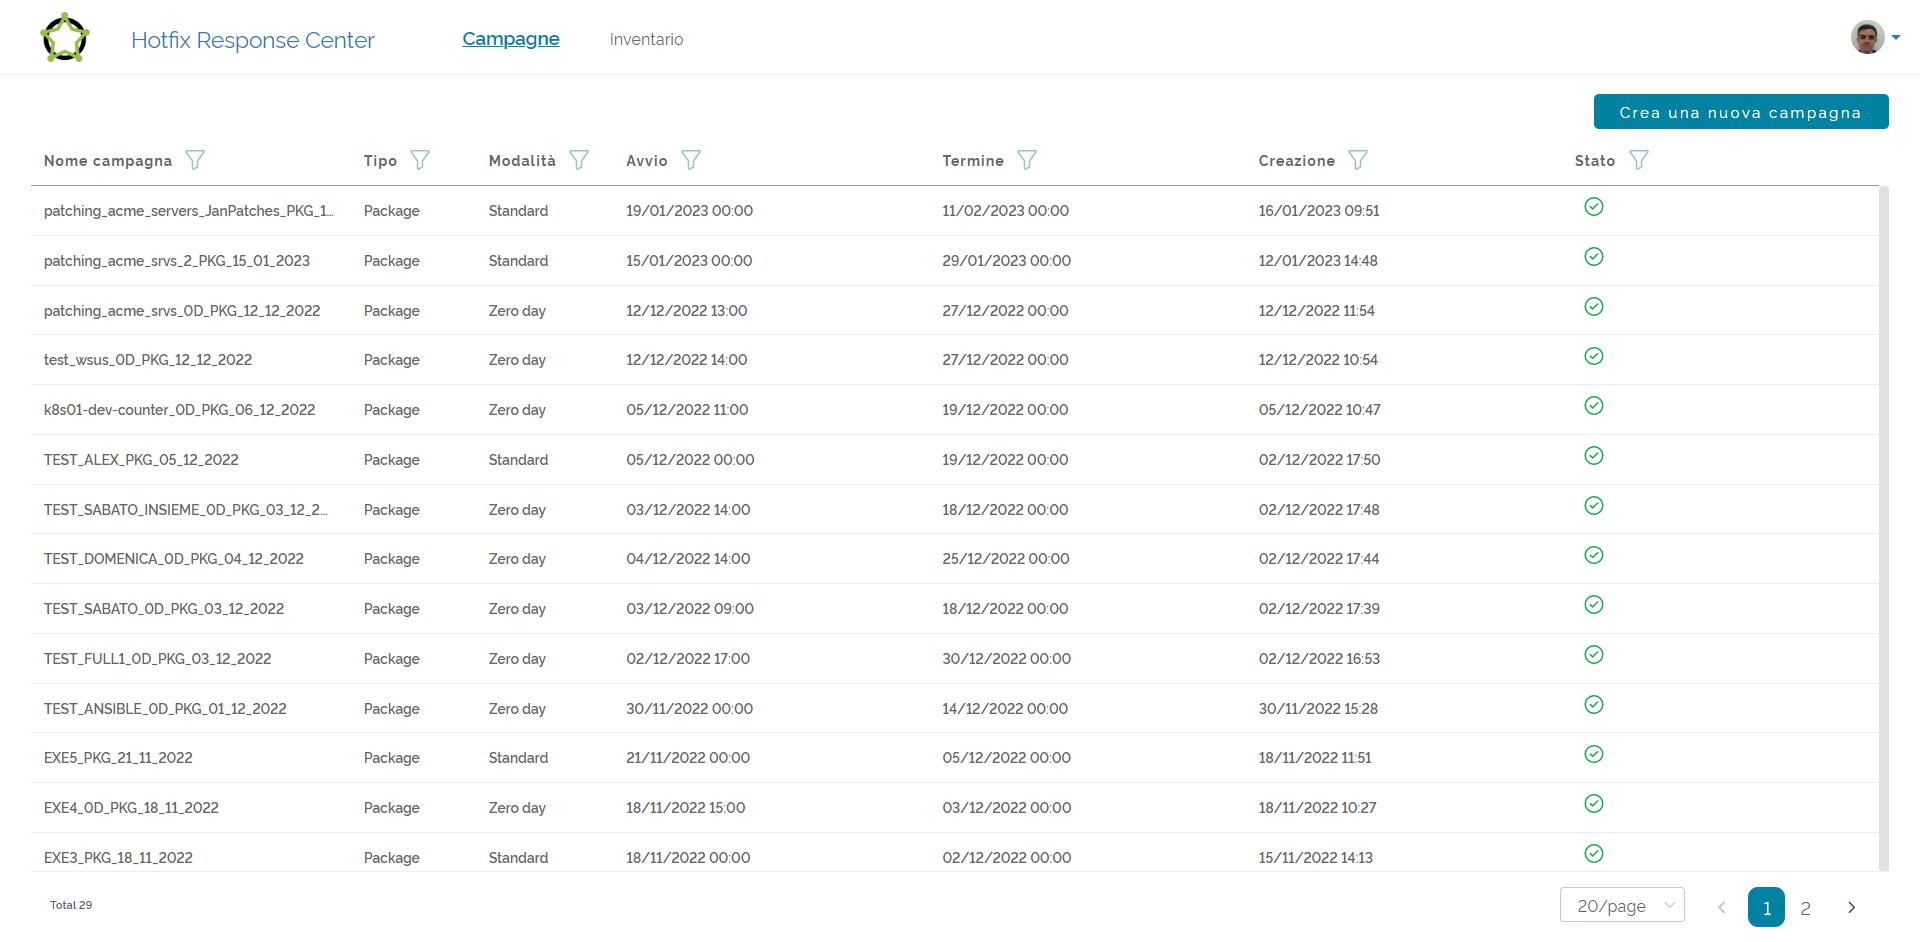
\includegraphics[width=0.98\textwidth]{imgs/ui/1_list_campaign.png}}
    \caption{Pagina principale, elenco delle campagne}
    \label{fig:Elenco delle campagne}
\end{flushright}
\end{figure}

Una volta che l'utente schiaccia il bottone per creare una nuova campagna, Vue.js 
esegue l'azione di click e carica dinamicamente la pagina specifica dedicata alla 
creazione della campagna. 

Questa pagina offre all'utente un'interfaccia intuitiva per inserire tutte 
le informazioni necessarie per avviare il processo di creazione 
della campagna. Attraverso questa pagina, l'utente può fornire le informazioni di base, 
come il nome della campagna, la modalità di esecuzione e le date di inizio e di 
fine.\\

Nella pagine successive verranno mostrate le schermate relative alla creazione di 
una campagna di aggiornamento su tutti i Windows Server di un cliente, per installare
un aggiornamento cumulativo rilasciato da Windows con identificativo KB5014850 che
serve a risolvere delle vulnerabilità di sistema.

\begin{figure}[H]
\begin{flushright}
    \centering
    \frame{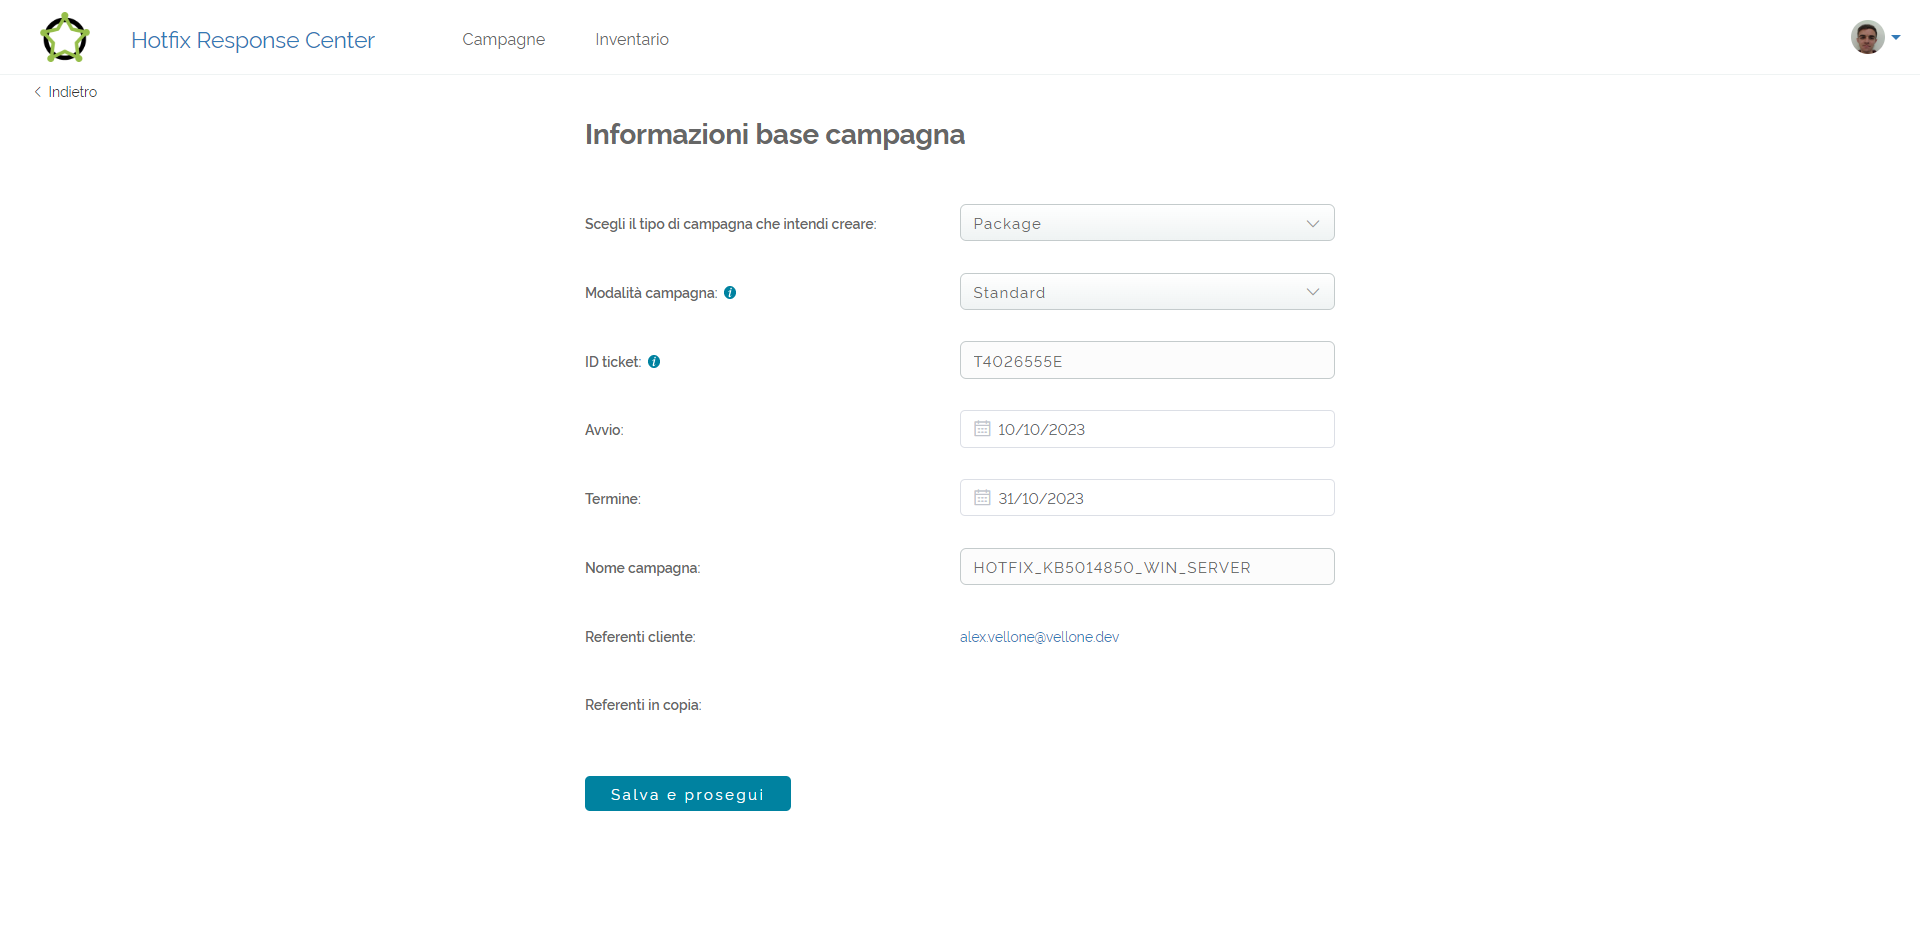
\includegraphics[width=0.95\textwidth]{imgs/ui/2_new_campagin.png}}
    \caption{Creazione di una nuova campagna}
    \label{fig:Creazione di una nuova campagna}
\end{flushright}
\end{figure}

Al click del bottone “Salva e prosegui” verrà eseguito il codice JavaScript per 
fare una chiamata POST alle API del backend con la quale verranno passate tutte le 
informazioni inserite dell’utente e verrà salvata la campagna all’interno del 
database.

Successivamente verrà mostrata la schermata per selezionare i server impattati 
dalla vulnerabilità. Da questa schermata è possibile utilizzare i filtri per 
selezionare rapidamente solo i server che si vogliono aggiornare.

\begin{figure}[H]
\begin{flushright}
    \centering
    \frame{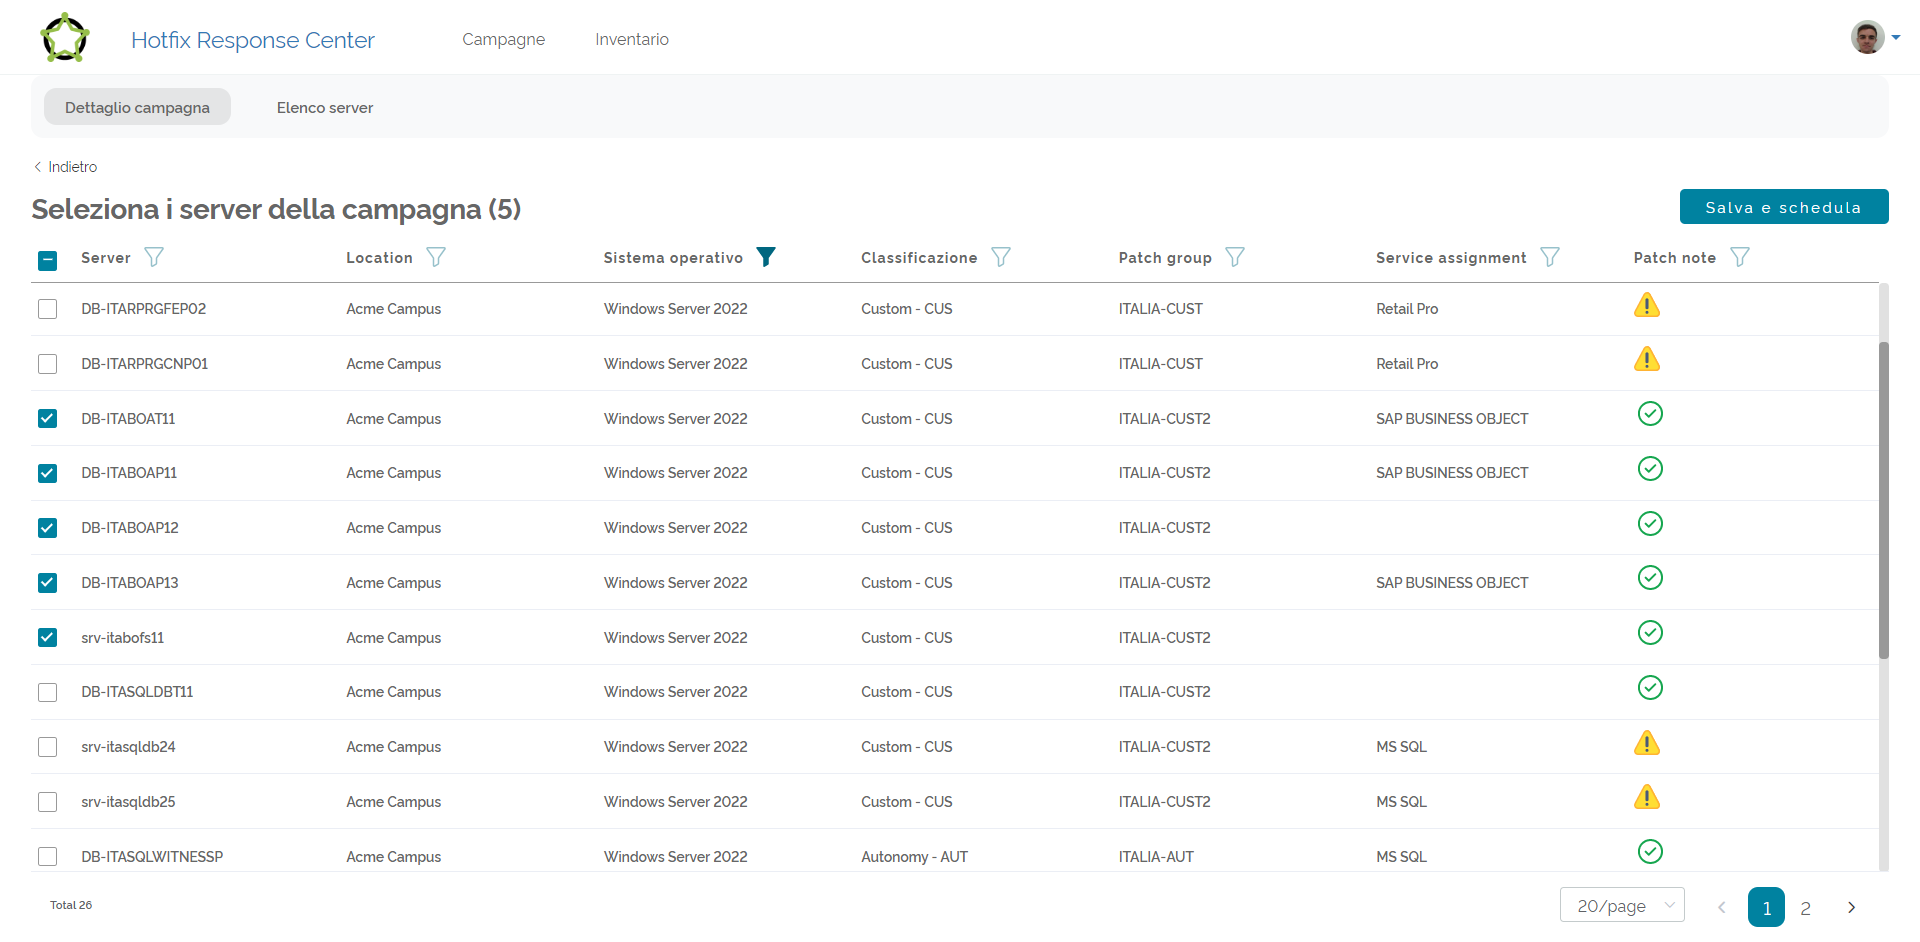
\includegraphics[width=0.95\textwidth]{imgs/ui/3_add_server.png}}
    \caption{Selezione elenco dei server impattati dalla vulnerabilità}
    \label{fig:Selezione elenco dei server impattati dalla vulnerabilità}
\end{flushright}
\end{figure}

Dopo aver selezionato tutti i server impattati sarà sufficiente fare click sul 
bottone “Salva e schedula” per inviare l’elenco dei server al backend, sempre 
tramite le API REST. 
Il backend avvierà a questo punto l’algoritmo di schedulazione per trovare uno
slot di manutenzione adatto per l'aggiornamento di tutti i server.

\begin{figure}[H]
\begin{flushright}
    \centering
    \frame{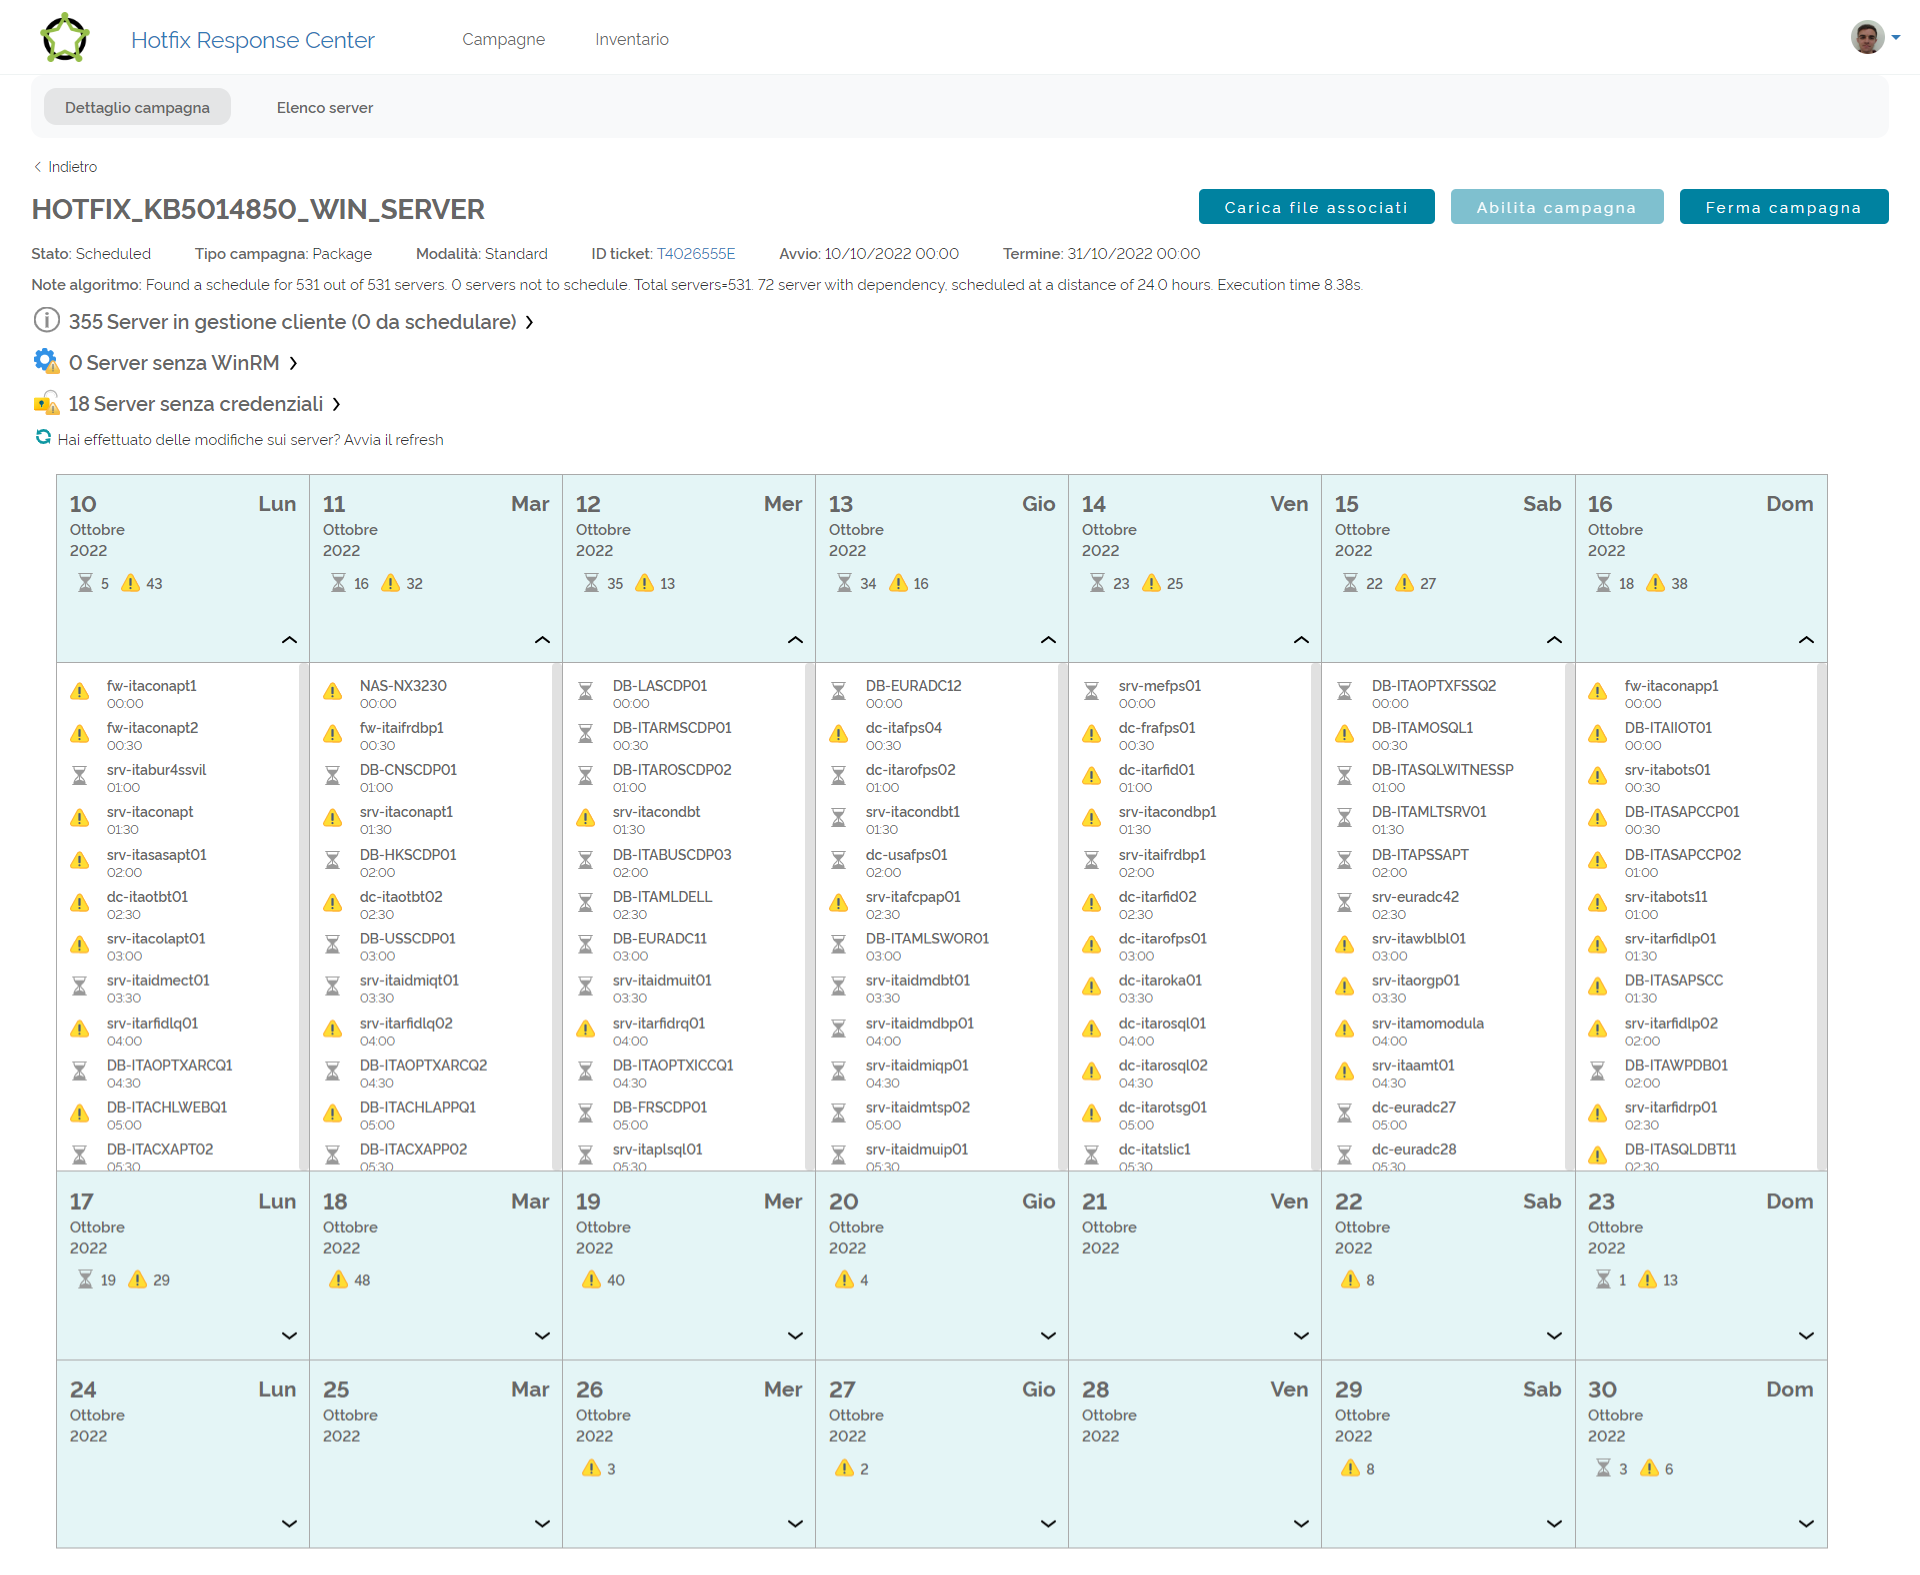
\includegraphics[width=0.98\textwidth]{imgs/ui/4_calendar.png}}
    \caption{Calendario della campagna}
    \label{fig:Calendario della campagna}
\end{flushright}
\end{figure}

Nella campagna selezionata sono stati inclusi 531 server, tutti pianificati con 
successo rispettando le rispettive finestre di manutenzione. Di questi, 72 sono 
stati considerati dipendenze e sono stati schedulati garantendo una separazione 
di 24 ore rispetto ai server di riferimento.

Per tutti i server della campagna è disponibile WinRM che consente quindi 
l'esecuzione automatica e remota degli aggiornamenti. Tuttavia, per 355 server 
è necessaria l'approvazione del cliente prima di procedere, mentre per 18 
server mancano le credenziali di connessione remota. Queste eccezioni sono 
segnalate nel calendario tramite un'icona di avviso, mentre per gli altri server 
gli aggiornamenti automatici partiranno nel rispettivo orario prestabilito.
I server con gli avvisi dovranno essere approvati per tempo dal cliente e 
l'operatore avrà del tempo per sistemare i problemi di credenziali sui 18 server.\\

Il calendario mostra un riepilogo, per ciascun giorno della campagna, 
consentendo di visualizzare i server schedulati nella giornata espandendo la 
settimana tramite un pulsante con una freccia verso il basso.

La pianificazione evidenzia in modo accurato come l'algoritmo abbia schedulato 
numerosi server nella prima settimana, riempiendo quasi completamente i 48 slot 
giornalieri disponibili. Nella terza settimana sono stati pianificati i server 
che presentano una programmazione più complessa a causa delle restrizioni imposte 
dalle finestre di manutenzione.\\

Prima dell'avvio della campagna, è necessario caricare i file di aggiornamento. 
In particolare, si mira a risolvere un gruppo di vulnerabilità nei sistemi 
operativi Windows Server utilizzando l'aggiornamento di sicurezza cumulativo 
con identificativo KB5014850, fornito da Microsoft.

Cliccando sul pulsante “Carica file associati”, si accede alla schermata dedicata 
al caricamento delle patch di sicurezza.

\begin{figure}[H]
\begin{flushright}
    \centering
    \frame{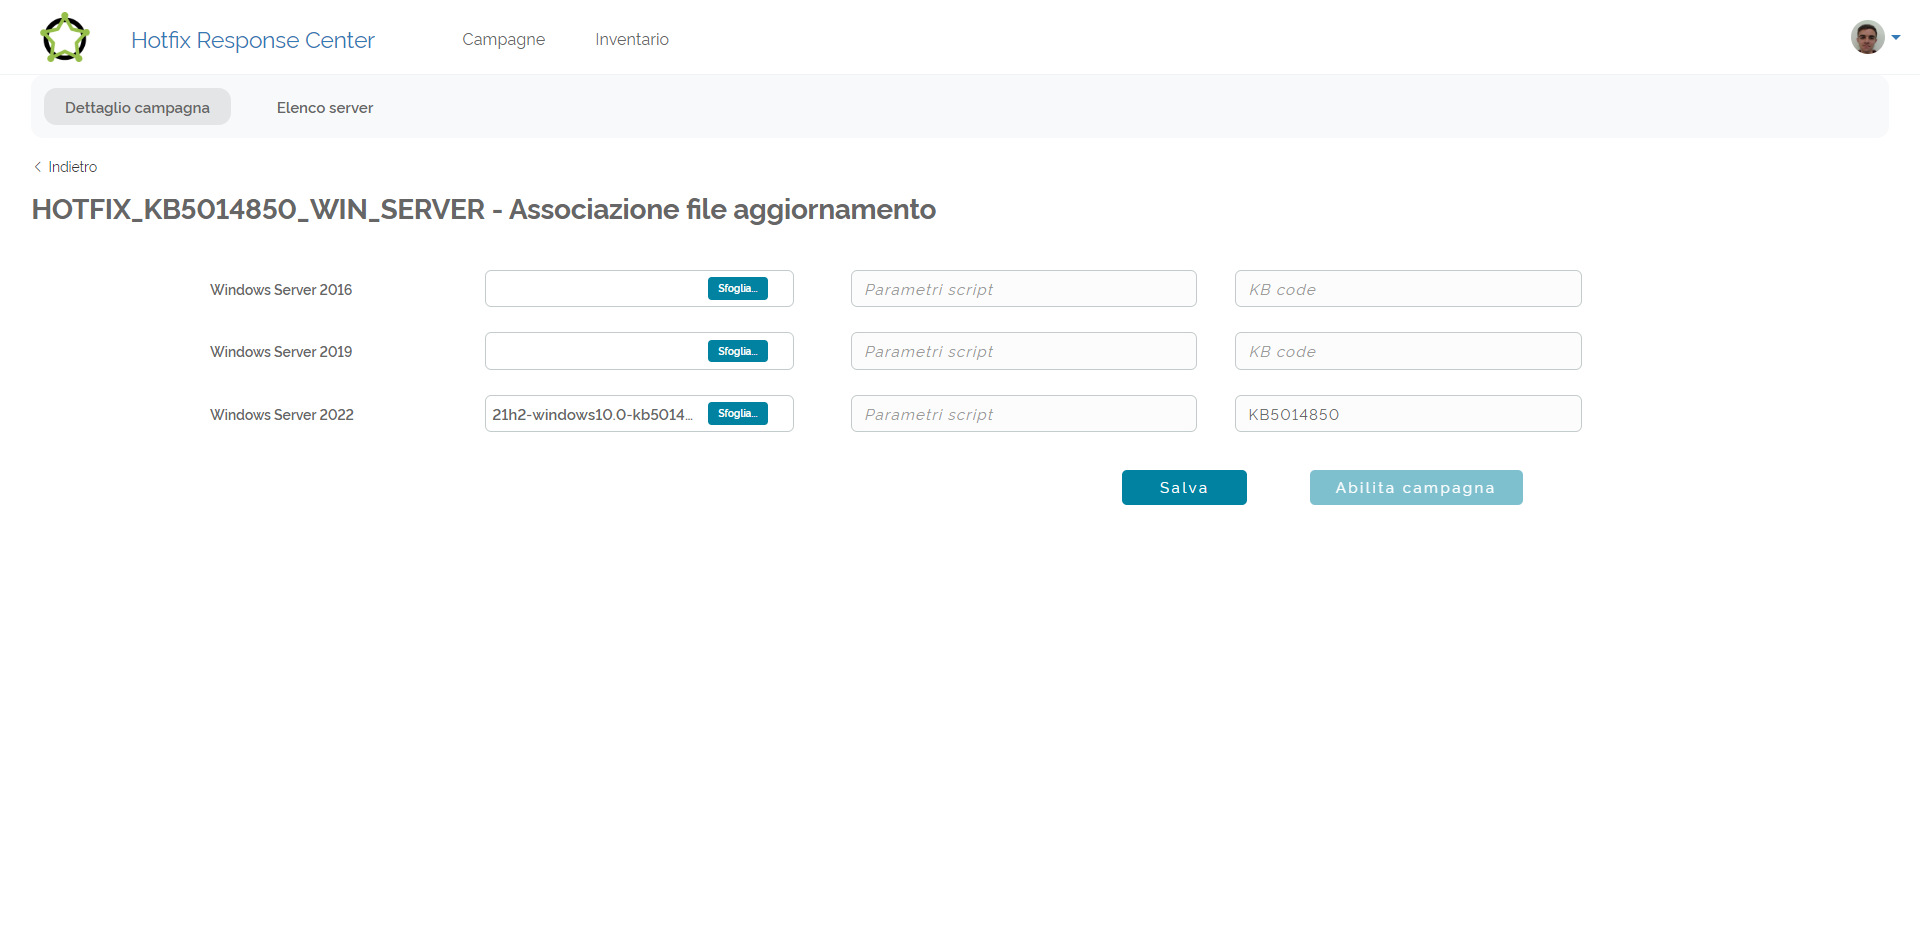
\includegraphics[width=0.98\textwidth]{imgs/ui/5_upload_files.png}}
    \caption{Upload dei file di aggiornamento}
    \label{fig:Upload dei file di aggiornamento}
\end{flushright}
\end{figure}

Considerando i 531 server selezionati, si rilevano tre diversi sistemi operativi: 
Windows Server 2016, Windows Server 2019 e Windows Server 2022. Per ognuno di 
questi sistemi operativi, è necessario caricare l'aggiornamento di sicurezza 
corretto, ottenibile dai canali ufficiali del fornitore del sistema operativo.

Una volta completato il caricamento, sarà possibile avviare la campagna mediante 
l'apposito pulsante “Abilita campagna”. Successivamente, l'Hotfix Response Center 
si occuperà dell'aggiornamento automatico e remoto dei server, eseguendo gli 
aggiornamenti secondo l'orario prestabilito.

\begin{figure}[H]
\begin{flushright}
    \centering
    \frame{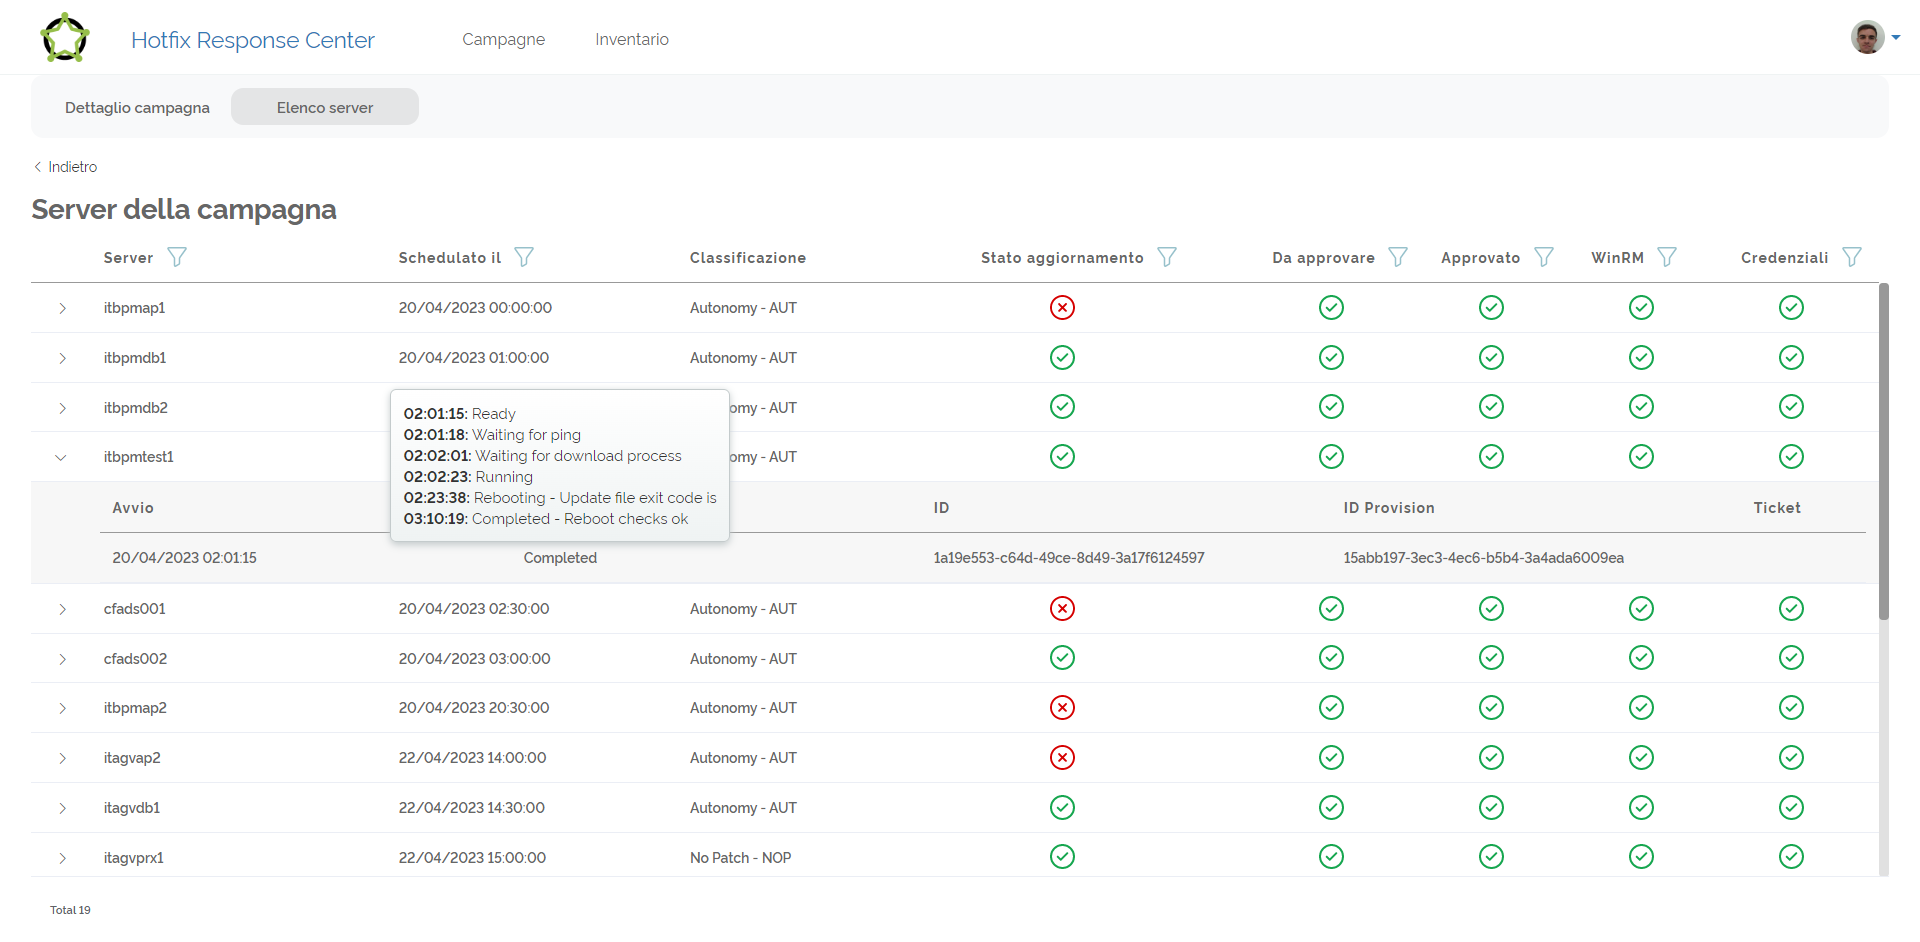
\includegraphics[width=0.98\textwidth]{imgs/ui/6_list_servers.png}}
    \caption{Elenco dei server della campagna}
    \label{fig:Elenco dei server della campagna}
\end{flushright}
\end{figure}

Attraverso la schermata “Elenco server”, è possibile visualizzare lo stato di 
aggiornamento di ogni singolo server. Tale stato può assumere quattro possibili 
valori: “Aggiornamento in attesa”, “Aggiornamento in corso”, “Completato” o “Fallito”.

Nel caso specifico di un aggiornamento fallito, è possibile utilizzare 
l'interfaccia del calendario per programmare manualmente una nuova data, al fine 
di tentare un aggiornamento automatico successivo. Tale funzionalità garantisce 
un'ulteriore opportunità per risolvere eventuali problemi e completare con 
successo l'aggiornamento del server interessato.\\

Nella maggior parte dei casi, l'aggiornamento risulta fallire a causa di server 
non raggiungibili o di credenziali di connessione non corrette. Quando ciò accade, 
è richiesto un intervento manuale per risolvere il problema prima di riprovare 
l'aggiornamento automatico. Per questo motivo si è deciso di lasciare all’operatore 
la decisione sulla scelta di una nuova data, per ritentare l'aggiornamento automatico.


\subsection{Conferma aggiornamento}
L’Hotfix Response Center è autonomamente in grado di riconoscere se 
l'aggiornamento è stato installato o meno sul server capendo anche se è 
necessario un riavvio per poterlo applicare correttamente.

In ogni caso, per verificare la corretta applicazione dell'aggiornamento di 
sicurezza applicato dalla campagna presa in analisi, è sufficiente collegarsi al 
server e verificare manualmente l’installazione lanciando il comando “Get-Hotfix” 
su una console Powershell con privilegi di amministratore.

\begin{figure}[H]
\begin{flushright}
    \centering
    \frame{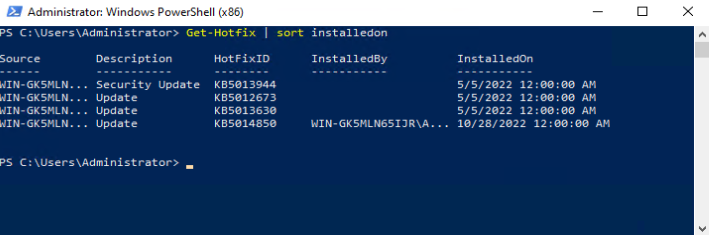
\includegraphics[width=0.98\textwidth]{imgs/ui/7_powershell_get_hotfix.png}}
    \caption{Console con il comando per verificare l'installazione dell'aggiornamento}
    \label{fig:Console con il comando per verificare l'installazione dell'aggiornamento}
\end{flushright}
\end{figure}

Nel server in questione possiamo notare che l'ultimo aggiornamento installato è
proprio l'aggiornamento cumulativo KB5014850 che conferma quindi l'installazione
remota e automatica dell'aggiornamento di sicurezza, attraverso la campagna di Hotfix.

  \mcchap{Conclusioni}{cap:cap5}

\section{Soluzioni già presenti sul mercato}
L'Hotfix Response Center è uno strumento realizzato da zero per adattarsi ad un 
contesto aziendale in cui ci sono già altri sistemi di patching in funzione. 
L'obiettivo era creare un tool indipendente dai sistemi aziendali già in uso, 
che potesse funzionare in modo semplice e soprattutto rapido in quanti più 
scenari possibili.\\

Esistono però diverse soluzioni simili ma più complete sul mercato. Un esempio è 
BigFix di IBM, un software che permette di gestire in maniera centralizzata 
le patch di sicurezza e le configurazioni di sistema di tutti i computer di una 
rete aziendale.
La soluzione BigFix di IBM si basa su un'architettura client-server in cui i 
dispositivi sono dotati di un agente che comunica costantemente con il server 
centrale. Questo permette alle organizzazioni di eseguire azioni di gestione e 
sicurezza su larga scala, come l'applicazione di patch, la distribuzione di software, 
la configurazione dei dispositivi e molto altro, in modo centralizzato e 
automatizzato. ~\cite{ibm:bigfix}

Sebbene BigFix offra funzionalità di gestione e sicurezza avanzate, è importante 
considerare alcuni fattori prima di adottarlo. In primo luogo, bisogna tenere 
presente che BigFix richiede l'acquisto di una licenza per ogni macchina gestita, 
il che può comportare costi significativi per le organizzazioni con un gran numero 
di server da gestire. Questo aspetto finanziario potrebbe influenzare la decisione 
di adottare BigFix come soluzione per la gestione delle sole patch.
Inoltre, per funzionare, BigFix ha bisogno di un suo agente funzionante sui server. 
L’agente è un applicativo da installare su ogni server che si vuole controllare. 
Il suo scopo è mantenere la comunicazione tra server e console centrale, in attesa 
di ricevere azioni da eseguire sul server gestito. L’installazione dell’agente può 
richiedere un impegno aggiuntivo in termini di tempo e risorse.

Soluzioni come BigFix offrono una vasta gamma di funzionalità di gestione e sicurezza, 
è però importante valutare attentamente i costi fissi di tale soluzione, le 
implementazioni e le esigenze specifiche dell'organizzazione.\\ 

L'Hotfix Response Center si propone di fornire una soluzione flessibile e semplice 
per la gestione delle patch senza però avere costi di gestione. L’Hotfix è stato 
progettato per essere indipendente dai sistemi aziendali già in uso e per funzionare 
in modo semplice e rapido in diversi scenari aziendali, solamente quando necessario. 
La sua flessibilità consente di adattarlo alle esigenze specifiche dell'organizzazione 
senza dover installare o mantenere nessun agente sul server che si vuole aggiornare.\\

In conclusione, mentre soluzioni come BigFix offrono una vasta gamma di funzionalità di 
gestione e sicurezza, è importante valutare attentamente i costi, le implementazioni e 
le esigenze specifiche dell'organizzazione prima di prendere una decisione. 
L'Hotfix Response Center si propone di fornire una soluzione, semplice e veloce per 
l’installazione degli aggiornamenti in situazioni di emergenza, in cui la rapidità è 
fondamentale. 
L’Hotfix Response Center può essere usato su tutti i server su cui è 
disponibile l’accesso remoto senza che sia necessario alcun software già installato 
sui server che si vuole aggiornare.

\section{Sviluppi futuri}
L’Hotfix Response Center rappresenta attualmente una soluzione efficace per la gestione in 
modo rapido delle campagne di aggiornamento, per risolvere le vulnerabilità. Tuttavia, per 
rendere il processo ancora più efficiente e automatizzato, sono in programma sviluppi futuri 
che introdurranno funzionalità avanzate.

Uno degli aspetti chiave in fase di sviluppo è la creazione automatica delle nuove campagne 
di aggiornamento. 
Attualmente, l'avvio delle campagne richiede un'azione manuale da parte degli operatori, che 
devono selezionare tutti i server impattati e caricare i file di aggiornamento. L'obiettivo 
è implementare una funzionalità che suggerisca automaticamente la creazione di nuove campagne 
in base alle informazioni raccolte da altri software interni all’azienda che recuperano 
l’elenco di tutti i software installati sui server.
Gli applicativi in questione monitorano costantemente i software installati sui server e 
inviano ad un database centrale tutte le informazioni recuperate.
Utilizzando le informazioni rese pubbliche dal NIST, all’interno del National Vulnerability 
Database, è possibile effettuare dei controlli di analisi proattiva per individuare se tra i 
software installati nei server dei clienti sono installati software con delle vulnerabilità.

Attraverso questo controllo incrociato l’Hotfix Response Center può suggerire agli 
amministratori di sistema la creazione di campagne per risolvere automaticamente le 
vulnerabilità presenti nei server impattati dalle vulnerabilità più gravi.\\

L'implementazione di questa funzionalità consentirà di automatizzare il processo di 
individuazione e gestione delle vulnerabilità, semplificando ulteriormente il lavoro degli 
amministratori di sistema e riducendo i tempi di risposta agli aggiornamenti critici. Ciò 
garantirà un ambiente più sicuro e protetto per le infrastrutture gestite.

Inoltre, l'Hotfix Response Center continuerà a essere sviluppato per integrarsi con altre 
piattaforme e strumenti utilizzati all'interno dell'azienda. L'obiettivo è creare un ecosistema 
completo che permetta una gestione centralizzata degli aggiornamenti, sfruttando 
al massimo le sinergie con i sistemi esistenti.\\

In conclusione, l'Hotfix Response Center è un progetto in continua evoluzione che mira a offrire 
soluzioni sempre più avanzate per la gestione delle campagne di aggiornamento. Grazie alle 
funzionalità future in fase di sviluppo, sarà possibile automatizzare il processo di 
individuazione e gestione delle vulnerabilità, migliorando la sicurezza e l'efficienza 
complessiva delle infrastrutture monitorate.


  \appendix
  %%\chapter*{Ringraziamenti}
\addcontentsline{toc}{chapter}{Ringraziamenti} % add it to the table of contents

\noindent Ringrazio i miei genitori per avermi cresciuto e per avermi costantemente supportato.
Ringrazio mio fratello Daniel, i miei nonni, gli zii e mio cugino per esserci sempre stati.\\

\noindent Ringrazio i miei compagni di corso con i quali ho condiviso questi anni di studio.
Ringrazio particolarmente Manuel per avermi tenuto sul pezzo anche quando non potevo 
seguire le lezioni universitarie.\\

\noindent Ringrazio i miei amici e le mie amiche che ho conosciuto in questi anni e 
con cui ho condiviso esperienze.\\

\noindent Ringrazio tutti i colleghi di Elmec Informatica S.p.A. con il quale ho 
lavorato negli ultimi quattro anni e che mi hanno aiutato a crescere professionalmente. 
Molto di quello che stato realizzato in questo progetto di tesi 
è stato fatto applicando le conoscenze acquisite lavorando insieme a loro.\\

\noindent Ringrazio il mio relatore nonché professore per la disponibilità e il 
rapido supporto durante la stesura di questa tesi.\\


  
  \backmatter{}

  %% Bibliografia
  \bibliography{biblio/biblio} 
  \bibliographystyle{ieeetr}

\end{document}
